% Options for packages loaded elsewhere
\PassOptionsToPackage{unicode}{hyperref}
\PassOptionsToPackage{hyphens}{url}
\PassOptionsToPackage{dvipsnames,svgnames,x11names}{xcolor}
%
\documentclass[
  10pt,
  a4paper,
]{article}
\usepackage{amsmath,amssymb}
\usepackage{iftex}
\ifPDFTeX
  \usepackage[T1]{fontenc}
  \usepackage[utf8]{inputenc}
  \usepackage{textcomp} % provide euro and other symbols
\else % if luatex or xetex
  \usepackage{unicode-math} % this also loads fontspec
  \defaultfontfeatures{Scale=MatchLowercase}
  \defaultfontfeatures[\rmfamily]{Ligatures=TeX,Scale=1}
\fi
% lmodern: not used (XeLaTeX with Latin Modern OpenType fonts)
\ifPDFTeX\else
  % xetex/luatex font selection
  \setmainfont[]{Latin Modern Roman}
\fi
% Use upquote if available, for straight quotes in verbatim environments
\IfFileExists{upquote.sty}{\usepackage{upquote}}{}
\IfFileExists{microtype.sty}{% use microtype if available
  \usepackage[]{microtype}
  \UseMicrotypeSet[protrusion]{basicmath} % disable protrusion for tt fonts
}{}
\makeatletter
\@ifundefined{KOMAClassName}{% if non-KOMA class
  \IfFileExists{parskip.sty}{%
    \usepackage{parskip}
  }{% else
    \setlength{\parindent}{0pt}
    \setlength{\parskip}{6pt plus 2pt minus 1pt}}
}{% if KOMA class
  \KOMAoptions{parskip=half}}
\makeatother
\usepackage{xcolor}
\usepackage[margin=2.3cm]{geometry}
\usepackage{longtable,booktabs,array}
\usepackage{calc} % for calculating minipage widths
% Correct order of tables after \paragraph or \subparagraph
\usepackage{etoolbox}
\makeatletter
\patchcmd\longtable{\par}{\if@noskipsec\mbox{}\fi\par}{}{}
\makeatother
% Allow footnotes in longtable head/foot
\IfFileExists{footnotehyper.sty}{\usepackage{footnotehyper}}{\usepackage{footnote}}
\makesavenoteenv{longtable}
\usepackage{graphicx}
\makeatletter
\def\maxwidth{\ifdim\Gin@nat@width>\linewidth\linewidth\else\Gin@nat@width\fi}
\def\maxheight{\ifdim\Gin@nat@height>\textheight\textheight\else\Gin@nat@height\fi}
\makeatother
% Scale images if necessary, so that they will not overflow the page
% margins by default, and it is still possible to overwrite the defaults
% using explicit options in \includegraphics[width, height, ...]{}
\setkeys{Gin}{width=\maxwidth,height=\maxheight,keepaspectratio}
% Set default figure placement to htbp
\makeatletter
\def\fps@figure{htbp}
\makeatother
\setlength{\emergencystretch}{3em} % prevent overfull lines
\providecommand{\tightlist}{%
  \setlength{\itemsep}{0pt}\setlength{\parskip}{0pt}}
\setcounter{secnumdepth}{5}

\usepackage{unicode-math}
\setmathfont{Latin Modern Math}
\usepackage{newunicodechar}
\newunicodechar{≥}{\ensuremath{\ge}}
\newunicodechar{≤}{\ensuremath{\le}}
\newunicodechar{≈}{\ensuremath{\approx}}
\newunicodechar{≠}{\ensuremath{\neq}}
\newunicodechar{∉}{\ensuremath{\notin}}
\newunicodechar{→}{\ensuremath{\rightarrow}}
\newunicodechar{×}{\ensuremath{\times}}
\newunicodechar{±}{\ensuremath{\pm}}
\newunicodechar{·}{\ensuremath{\cdot}}
\newunicodechar{Σ}{\ensuremath{\Sigma}}
\newunicodechar{τ}{\ensuremath{\tau}}
\newunicodechar{γ}{\ensuremath{\gamma}}
\usepackage{booktabs}
\usepackage{microtype}
\usepackage{xurl}
\setlength{\LTcapwidth}{\linewidth}
\usepackage[font=small,labelfont=bf]{caption}
\usepackage{etoolbox}
\AtBeginEnvironment{longtable}{\small\renewcommand{\arraystretch}{1.12}}
\renewcommand{\floatpagefraction}{0.8}
\renewcommand{\topfraction}{0.9}
\newcommand{\lbl}[1]{\texttt{#1}}
\ifLuaTeX
  \usepackage{selnolig}  % disable illegal ligatures
\fi
\IfFileExists{bookmark.sty}{\usepackage{bookmark}}{\usepackage{hyperref}}
\IfFileExists{xurl.sty}{\usepackage{xurl}}{} % add URL line breaks if available
\urlstyle{same}
\hypersetup{
  pdftitle={Which forks? The definition of a forking token can flip its relation to entropy},
  colorlinks=true,
  linkcolor={blue},
  filecolor={Maroon},
  citecolor={Blue},
  urlcolor={blue},
  pdfcreator={LaTeX via pandoc}}

\title{Which forks? The definition of a forking token can flip its relation to entropy}
\author{Chisa Honda\\[2pt] {\small Independent researcher}}
\date{Draft, November 2026}

\begin{document}
\maketitle

\begin{abstract}

Token-level entropy is widely used to find the ``forking tokens'' of chain-of-thought reasoning: positions where a different choice would change the outcome. A fork can be measured by forcing an
alternative token (a \emph{forced swap}) or by \emph{resampling} from the position. We measure both at the same positions, in a series of mostly pre-registered experiments with replay audits, on
GSM-Symbolic arithmetic with three open models (OLMo-2 1B, Gemma-2-2b-it and Qwen2.5-7B-Instruct). On these models, entropy relates to the two definitions in opposite directions. Large forced-swap
effects concentrate on confident, answer-bearing digit tokens (a substantial part of the pattern, not all of it), so entropy points away from them (within-item AUROC 0.20--0.42 in five experiments;
confirmed under pre-registration in four). In Gemma this persisted when the swapped-in token's probability was held near \(10^{-6}\), so it is not only an effect of swapping in improbable tokens.
Large resampling drops, estimated with a stratified estimator, align with entropy (0.75--0.89), but largely by construction: the drop factors exactly as
\((1-p_1)\)(\(q_{\mathrm{alt}} - q_{\mathrm{keep}}\)), and keeping each position's 1 − \(p_1\) while shuffling the effects reproduces the alignment (post hoc, in the two smaller models). The same
identity gives a lower-variance estimator of the drop. The two views meet at rare alternatives: in Gemma, an alternative the model itself samples at a confident position was about as damaging as a
forced one, but such positions contributed almost nothing to how sampled answers vary. On a synthetic name-lookup task (Gemma, one hop) the anti-alignment did not appear. In the 7B model, six of seven
pre-registered tests came out as predicted; the resampling side was only weakly measured there, and the test of rare positions was undecided. Studies that use entropy as a forking signal should state
which definition they need and report answer-bearing tokens separately.

\end{abstract}

\hypertarget{introduction}{%
\section{Introduction}\label{introduction}}

High-entropy tokens have been proposed as the ``forks'' of reasoning: the minority of positions where the model hesitates, and where training signal or analysis should concentrate (Wang et al., 2025;
Cheng et al., 2026). Direct tests of whether such positions change outcomes use two operationalisations:

\begin{itemize}
\tightlist
\item
  \textbf{Forced swap.} Replace the chosen token with an alternative (typically the runner-up) and check whether the answer changes (Ruan et al., 2025; at the sentence level, off-policy edits in Macar
  et al., 2026).
\item
  \textbf{Resampling.} Sample the token and its continuation from a prefix and measure how the answer distribution moves (at the sentence level, Bogdan et al., 2025; Macar et al., 2026). Forking Paths
  (Bigelow et al., 2025) combines the two: it forces each probable alternative token, samples continuations after it, and weights the outcomes by the token's probability.
\end{itemize}

A forced swap asks \emph{``what if this token were different?''}, ignoring how likely that is. Resampling asks \emph{``does the outcome actually branch here?''}, which combines the effect of an
alternative with the chance of sampling one. We show that on arithmetic this difference reverses the direction of entropy's relation to forks, and we take the reversal apart. One half of it is built
into the resampling definition. The other half is the empirical finding: forced-swap effects concentrate on confident, answer-bearing digit tokens. That digits matter in arithmetic is not surprising;
what matters for entropy-based methods is that, under one definition, selecting tokens by entropy systematically passes over them.

\textbf{Findings.}

\begin{enumerate}
\def\labelenumi{\arabic{enumi}.}
\tightlist
\item
  \textbf{Forced-swap effects sit at confident digit tokens (§3.1, §3.3).} Entropy is anti-aligned with these effects in all five arithmetic experiments, and the anti-alignment was confirmed under
  pre-registration in four, on three models (1.5B to 7.6B parameters, three families). Digit tokens carry a substantial part of it, not all. In Gemma it persisted when the probability of the
  swapped-in token was fixed at about \(10^{-6}\) at every position, although the matched token at a digit position was often itself a digit. On a synthetic name-lookup task it did not appear (§3.4),
  so it may be specific to arithmetic.
\item
  \textbf{The resampling side is largely built in (§3.2).} The resampling drop factors exactly into the chance that an alternative is sampled, 1 − \(p_1\), times the effect of an alternative. A
  baseline that keeps 1 − \(p_1\) and shuffles the effects within items reproduces entropy's alignment with the drop (post hoc). That alignment is largely a property of the definition, not a finding
  about where reasoning branches.
\item
  \textbf{Rare alternatives (§3.5).} In Gemma, an alternative that the model itself samples was about as damaging as the forced runner-up, and most damaging where alternatives are rarest; but such
  positions contributed almost nothing to how the answer varies under sampling. Our reading (an interpretation, not a registered test) is that the two definitions look at the same positions from
  opposite sides.
\item
  \textbf{A larger model of a third family (§3.6).} In Qwen2.5-7B-Instruct the anti-alignment, the weighting, the digit concentration and the first two rarity results replicated under the original
  decision rules. The alignment with the resampling drop was confirmed under a new rule but only weakly measured, probably because that model leaves almost no drop at most positions. Whether rare
  positions contribute little was undecided, and the probability-matched swap was made descriptive before the run (a smoke run had found a token near \(10^{-6}\) at only 47\% of positions).
\end{enumerate}

\textbf{Contributions.} (a) A same-position, within-item comparison of entropy against both fork definitions (five experiments, three model families), within a series of ten pre-registered experiments
with frozen decision rules and replay audits; every registered test and its outcome, including negative results such as a transcoder study (Appendix C), is listed in Appendix B. (b) An exact
decomposition that explains the resampling side and a weight-only baseline that shows how much of it is built in. (c) A probability-matched swap that separates ``the model is confident here'' from
``the swapped-in token is improbable''. (\(d\)) A same-position comparison of natural and forced alternatives across bands of rarity, which separates the size of an effect from its contribution to
answer variation. (\(e\)) A practical tool: a stratified estimator of the resampling drop that makes per-position estimates usable at feasible sample sizes.

\hypertarget{setup}{%
\section{Setup}\label{setup}}

\textbf{Models.}

\begin{itemize}
\tightlist
\item
  OLMo-2 1B (\texttt{allenai/OLMo-2-0425-1B-Instruct}; Team OLMo et al., 2025; fixed revision, float16).
\item
  Gemma-2-2b-it (\texttt{google/gemma-2-2b-it}; Gemma Team, 2024; fixed revision, bfloat16, eager attention).
\item
  Qwen2.5-7B-Instruct (\texttt{Qwen/Qwen2.5-7B-Instruct}; Qwen Team, 2024; fixed revision, bfloat16, PyTorch's scaled-dot-product attention), used only in the replication DP9 (§3.6). Its own chat
  template, which inserts a default system message, is used unchanged.
\end{itemize}

\textbf{Data.} GSM-Symbolic (Mirzadeh et al., 2025). Each experiment uses items not used in any earlier experiment of this series, except one transcoder study (CT-1, Table 1), which reused the items
of a resampling experiment (DP2) by design. Earlier draws are reconstructed and excluded before any token is generated. Templates may repeat across experiments. One experiment (DP6) instead uses a
synthetic name-lookup task (§3.4).

\textbf{Experiments.} Table 1 lists the experiments. We refer to them by their short names; the results are organised by claim, not by experiment.

\begin{longtable}[]{@{}
  >{\raggedright\arraybackslash}p{(\columnwidth - 8\tabcolsep) * \real{0.0776}}
  >{\raggedright\arraybackslash}p{(\columnwidth - 8\tabcolsep) * \real{0.1746}}
  >{\raggedright\arraybackslash}p{(\columnwidth - 8\tabcolsep) * \real{0.1649}}
  >{\raggedright\arraybackslash}p{(\columnwidth - 8\tabcolsep) * \real{0.3589}}
  >{\raggedright\arraybackslash}p{(\columnwidth - 8\tabcolsep) * \real{0.1940}}@{}}
\caption{The experiments, in the order they were run (the closed-model studies of Appendices D and E and the Japanese check of Appendix F are not listed).}\tabularnewline
\toprule\noalign{}
\begin{minipage}[b]{\linewidth}\raggedright
Name
\end{minipage} & \begin{minipage}[b]{\linewidth}\raggedright
Model
\end{minipage} & \begin{minipage}[b]{\linewidth}\raggedright
Items run / analysed
\end{minipage} & \begin{minipage}[b]{\linewidth}\raggedright
What it measures
\end{minipage} & \begin{minipage}[b]{\linewidth}\raggedright
Status
\end{minipage} \\
\midrule\noalign{}
\endfirsthead
\toprule\noalign{}
\begin{minipage}[b]{\linewidth}\raggedright
Name
\end{minipage} & \begin{minipage}[b]{\linewidth}\raggedright
Model
\end{minipage} & \begin{minipage}[b]{\linewidth}\raggedright
Items run / analysed
\end{minipage} & \begin{minipage}[b]{\linewidth}\raggedright
What it measures
\end{minipage} & \begin{minipage}[b]{\linewidth}\raggedright
Status
\end{minipage} \\
\midrule\noalign{}
\endhead
\bottomrule\noalign{}
\endlastfoot
DP1 & OLMo-2 1B & 100 / 100 & forced-swap forks (greedy continuation) & pre-registered \\
DP2 & OLMo-2 1B & 60 / 60 & resampling forks over 8-token windows & pre-registered \\
DP3 & OLMo-2 1B & 40 / 39 & both definitions at the same positions; digits & pre-registered \\
CT-1 & Gemma-2-2b-it & DP2's items (56 pairs) & transcoder explanation of forks (Appendix C) & pre-registered \\
DP4 & OLMo-2 1B & 40 / 40 & both definitions, stratified drop & pre-registered \\
DP5 & Gemma-2-2b-it & 40 / 39 & replication on a second model; digit source & pre-registered \\
DP6 & Gemma-2-2b-it & 40 / 40 & name lookup instead of arithmetic & pre-registered \\
R1 & --- & records of DP3--DP6 & weight-only baseline, swap size, readout, robustness & post hoc (frozen plan) \\
DP7 & Gemma-2-2b-it & 40 / 39 & probability-matched forced swap & pre-registered \\
DP8-X & --- & records of DP4, DP5, DP7 & effects of natural and forced alternatives by rarity & post hoc (views fixed in advance) \\
DP8 & Gemma-2-2b-it & 40 / 38 & natural versus forced alternatives by rarity & pre-registered \\
DP9 & Qwen2.5-7B-Instruct & 40 / 39 & replication of DP5 and DP8 on a larger model of a third family & pre-registered \\
\end{longtable}

\textbf{Base path.} Greedy decoding (ties to the lower token id), at most 512 tokens. The answer is taken from the final-answer line, falling back to the last number (DP6: a name read from the
final-answer line); numbers are compared exactly. Items whose base answer cannot be read are excluded. We analyse positions before the first answer token a (the token that contains the first character
of the answer): in DP3--DP9, every 4th (DP3), 6th (DP4) or 8th (DP5--DP9) token from the start of the response. A \emph{digit position} is one whose base-path token contains a digit.

\textbf{Fork quantities (Figure 1).} At position \(t\), let \(w_1\) be the top token (with probability \(p_1\)) and \(w_2\) the runner-up (\(p_2\)). We fix the token at \(t\) and sample \(K\)
continuations at temperature 1.0 (\(K = 32\) in DP3--DP9). Let \(q\) be the fraction of continuations whose answer differs from the base answer; an unreadable answer counts as different.

\begin{itemize}
\tightlist
\item
  \emph{Forced-swap effect}: \(e(t) = q_{\mathrm{swap}}(t) - q_{\mathrm{keep}}(t)\), with the token at \(t\) fixed to \(w_2\) versus \(w_1\).
\item
  \emph{Probability-matched swap effect (DP7)}: \(e_\tau(t) = q_{\mathrm{swap}\tau}(t) - q_{\mathrm{keep}}(t)\), with the token at \(t\) fixed to \(w_{\tau}\), the token whose probability at \(t\) is
  closest to \(\tau = 10^{-6}\) in log space (\(w_1\), end-of-sequence and special tokens excluded; \(w_2\) allowed; ties to the lower id). A position is \emph{matched} if \(p\)(\(w_{\tau}\)) lies
  within ±0.5 decades of \(\tau\).
\item
  \emph{Forced fork (DP1, DP3)}: the single greedy continuation after the swap changes the answer.
\item
  \emph{Resampling drop}: \(d(t) = q_{\mathrm{free}}(t) - q_{\mathrm{keep}}(t)\), where ``free'' also samples the token at t. \(d\) is how much the chance of a changed answer falls once the token at
  \(t\) is fixed to the greedy choice, that is, how much of the outcome is decided at t. DP2 uses a window version, \(q(t) - q(t+8)\), with 16 samples.
\end{itemize}

\textbf{Stratified drop.} Sampling the token at \(t\) from the model's own distribution gives exactly

\[q_{\mathrm{free}} = p_1\,q_{\mathrm{keep}} + (1-p_1)\,q_{\mathrm{alt}},\qquad\text{so}\qquad d = (1-p_1)\,(q_{\mathrm{alt}}-q_{\mathrm{keep}}),\]

where \(q_{\mathrm{alt}}\) samples the token at \(t\) with \(w_1\) removed and the rest renormalised. The identity holds for the underlying probabilities, up to numerical differences between the
logits used for \(p_1\) and those used for sampling (Appendix A).

\begin{itemize}
\tightlist
\item
  \(d_{s} = (1-p_1) \cdot e_{\mathrm{alt}}\), with \(e_{\mathrm{alt}} = q_{\mathrm{alt}} - q_{\mathrm{keep}}\) (the effect of replacing \(w_1\) by a sampled alternative), is unbiased for d.
\item
  \(p_1\) is read off the logits rather than sampled, so the variance of \(d_{s}\) is \((1-p_1)\)² times that of the estimated \(e_{\mathrm{alt}}\). Its standard deviation shrinks in proportion to 1 −
  \(p_1\) at confident positions; that of the plain estimate does not.
\item
  It needs the same number of samples as the plain estimate (keep + alt instead of keep + free).
\end{itemize}

Conditioning on the first token and reweighting follows Forking Paths (Bigelow et al., 2025), whose outcome distribution is a mixture over alternative tokens weighted by their probabilities; \(d_{s}\)
is its two-group case (the greedy token versus all others). Using the exact probability of the greedy category instead of sampling which category occurs is a form of Rao--Blackwellization (cf.~Liu et
al., 2019). More generally, Re et al. (2026) use the next-token distributions available during sampling to reduce the variance of expectation estimates under language models; the stratified drop
applies this idea at a single position with two strata. The identity itself is an application of the law of total expectation. At the sentence level, Thought Anchors makes the analogous split between
resampling importance and counterfactual importance (Bogdan et al., 2025). We claim no novelty for any of these, only for using the \((1-p_1)\) factor to explain the entropy relation (Appendix A).

\begin{figure}
\centering
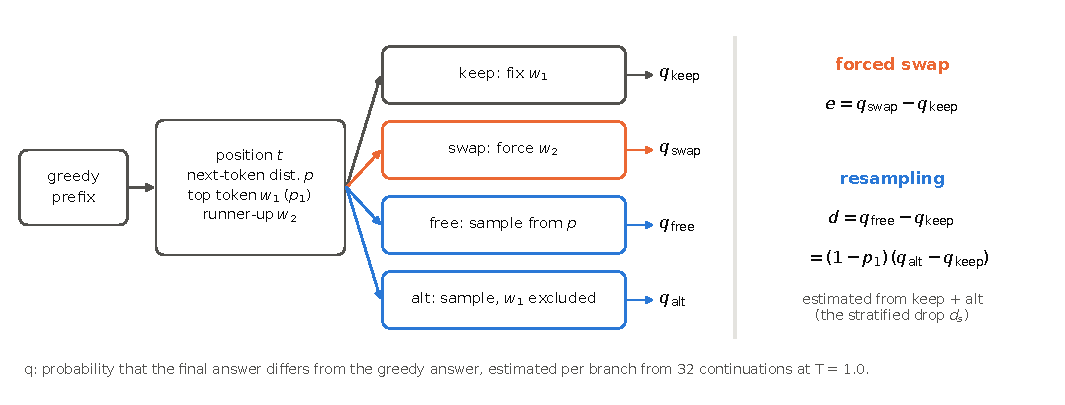
\includegraphics{../figures/fig1_definitions.pdf}
\caption{The two definitions of a forking token. At position \(t\) of the greedy path, the token is fixed to the top token \(w_1\) (keep) or to the runner-up \(w_2\) (swap), or it is sampled from the
model's distribution, either in full (free) or with \(w_1\) excluded (alt). Each \(q\) is the probability that the final answer differs from the greedy answer, estimated from 32 continuations at
temperature 1.0 (DP3--DP9). The forced-swap effect \(e\) compares swap with keep; the resampling drop \(d\) compares free with keep, and the identity on the right holds for these probabilities. DP3
ran keep, swap and free and used the plain estimate of d.~DP4--DP6 ran keep, swap and alt at every position and rank positions by the stratified drop \(d_{s}\), estimated from keep and alt; free was
run only to check this estimator and its noise (at every position in DP4, at every third position in DP5 and DP6). DP7 ran keep, swap and a third forced swap to a token of probability about
\(10^{-6}\) (not shown); DP8 ran keep, swap, alt and that swap at every position (§3.5); DP9 ran the same four at every position and free at every third (§3.6).}
\end{figure}

\textbf{Evaluation.}

\begin{itemize}
\tightlist
\item
  Labels are the top 15\% of all positions in an experiment (pooled across items) by \(e\), \(e_{\tau}\), \(d\) (DP3), \(e_{\mathrm{alt}}\) or \(d_{s}\); in DP7, among matched positions only. Ties at
  the cut are broken by item order, then position.
\item
  The score is the next-token entropy at \(t\) in nats, computed from the temperature-1.0 distribution that is sampled from (after soft-capping for Gemma).
\item
  We report the within-item AUROC: computed per item that has both classes, then averaged with equal weight per item. Items with no labelled position (or only labelled positions) drop out, so each
  estimate rests on fewer items than were run (for example 36 of 39 for top \(e\) in DP5), and a difference between two AUROCs can average over slightly different sets of items.
\item
  CIs are 95\% percentile bootstrap intervals with 2,000 resamples of templates, labels held fixed; DP3--DP5, DP7--DP9 drew one item per template, and DP6 resamples items (each has its own roster).
  Differences use the same resamples. Intervals are per comparison and not adjusted for multiple comparisons.
\item
  DP8 does not label positions. Its tests are position-weighted mean differences, a ratio of sums and a mean within-item Spearman correlation (§3.5), with intervals from the same item bootstrap; items
  whose base answer cannot be read have no positions and enter only the base accuracy. DP9 repeats DP5's labelled tests and DP8's first three tests with the same definitions, and adds one new test
  (§3.6).
\end{itemize}

\textbf{Pre-registration and audit.}

\begin{itemize}
\tightlist
\item
  Each confirmatory experiment (DP1--DP9 and CT-1) had a gate document fixing definitions, seeds, labels and decision thresholds. It was frozen and hashed before running. Appendix B lists every
  decision rule and its outcome.
\item
  R1 is a set of post hoc analyses of existing records, run from a plan frozen before computing them; we label its results ``post hoc''. Other exploratory analyses (DP1-X, DP1-X2, DP2-X1, DP2-X2, the
  DP2 side analyses and DP3-X1, DP8-X; described in Appendix B) are also marked post hoc. Analyses that a gate lists as secondary but without a decision rule are called pre-specified secondary
  analyses.
\item
  After each confirmatory run, a replay audit regenerated a pre-declared subset of outputs with reference implementations: base paths, continuations or samples on 5--10 items (in DP7--DP9 also the
  choice of \(w_{\tau}\), in DP8 and DP9 also the first token of alt, in DP9 also free). Every audit matched (0 diverged items).
\item
  In the main text we state each registered outcome in words (confirmed, not confirmed, not replicated or undecided under its rule). The frozen rules and the registered outcome labels are listed in
  Appendix B (Table 8). ``Label'' in the main text always means membership in the top 15\% of positions.
\end{itemize}

\textbf{Origins.} The series began with one definition per experiment on OLMo-2 1B: forced swaps (DP1) and resampling over 8-token windows (DP2). Within items, entropy was anti-aligned with
forced-swap forks (post hoc) and moderately aligned with resampling forks, and a post hoc look at DP1's records suggested that weighting by the runner-up's probability nearly reproduced the gap. These
observations motivated DP3--DP5 (Appendix G).

\hypertarget{results}{%
\section{Results}\label{results}}

\hypertarget{forced-swap-effects-are-anti-aligned-with-entropy-on-arithmetic}{%
\subsection{Forced-swap effects are anti-aligned with entropy on arithmetic}\label{forced-swap-effects-are-anti-aligned-with-entropy-on-arithmetic}}

At the same positions, entropy's within-item AUROC for the top 15\% of forced-swap effects lies below 0.5 in every arithmetic experiment (Table 2, Figure 2). Comparing it with 0.5 was a registered
test in DP4, DP5, DP7 (where the runner-up swap was the prerequisite test) and DP9, and post hoc in DP3.

\begin{longtable}[]{@{}
  >{\raggedright\arraybackslash}p{(\columnwidth - 8\tabcolsep) * \real{0.2013}}
  >{\raggedright\arraybackslash}p{(\columnwidth - 8\tabcolsep) * \real{0.1971}}
  >{\raggedright\arraybackslash}p{(\columnwidth - 8\tabcolsep) * \real{0.1482}}
  >{\raggedright\arraybackslash}p{(\columnwidth - 8\tabcolsep) * \real{0.1838}}
  >{\raggedright\arraybackslash}p{(\columnwidth - 8\tabcolsep) * \real{0.2396}}@{}}
\caption{Entropy's within-item AUROC under each definition, with 95\% CIs. Registered outcomes for top \(e\): anti-alignment confirmed in DP4, DP5, DP7 and DP9, not replicated in DP6. For top
\(d_{s}\), alignment was a registered test only in DP9 (confirmed); in DP4--DP6 this value entered only the weighting test.}\tabularnewline
\toprule\noalign{}
\begin{minipage}[b]{\linewidth}\raggedright
Experiment
\end{minipage} & \begin{minipage}[b]{\linewidth}\raggedright
Model, items analysed
\end{minipage} & \begin{minipage}[b]{\linewidth}\raggedright
Positions
\end{minipage} & \begin{minipage}[b]{\linewidth}\raggedright
Entropy AUROC, top \(e\)
\end{minipage} & \begin{minipage}[b]{\linewidth}\raggedright
Entropy AUROC, top resampling drop
\end{minipage} \\
\midrule\noalign{}
\endfirsthead
\toprule\noalign{}
\begin{minipage}[b]{\linewidth}\raggedright
Experiment
\end{minipage} & \begin{minipage}[b]{\linewidth}\raggedright
Model, items analysed
\end{minipage} & \begin{minipage}[b]{\linewidth}\raggedright
Positions
\end{minipage} & \begin{minipage}[b]{\linewidth}\raggedright
Entropy AUROC, top \(e\)
\end{minipage} & \begin{minipage}[b]{\linewidth}\raggedright
Entropy AUROC, top resampling drop
\end{minipage} \\
\midrule\noalign{}
\endhead
\bottomrule\noalign{}
\endlastfoot
DP3 & OLMo-2 1B, 39 & 1,692 & 0.415 {[}0.353, 0.482{]} & 0.558 {[}0.495, 0.620{]} (plain \(d\)) \\
DP4 & OLMo-2 1B, 40 & 1,046 & 0.378 {[}0.316, 0.440{]} & 0.887 {[}0.862, 0.911{]} (\(d_{s}\)) \\
DP5 & Gemma-2-2b-it, 39 & 905 & 0.286 {[}0.211, 0.370{]} & 0.858 {[}0.821, 0.891{]} (\(d_{s}\)) \\
DP7 & Gemma-2-2b-it, 39 & 811 (matched) & 0.203 {[}0.160, 0.246{]} & --- (not measured) \\
DP9 (§3.6) & Qwen2.5-7B-Instruct, 39 & 1,324 & 0.259 {[}0.200, 0.321{]} & 0.745 {[}0.703, 0.786{]} (\(d_{s}\)) \\
DP6 (name lookup, §3.4) & Gemma-2-2b-it, 40 & 388 & 0.574 {[}0.488, 0.658{]} & 0.860 {[}0.807, 0.906{]} (\(d_{s}\)) \\
\end{longtable}

\begin{figure}
\centering
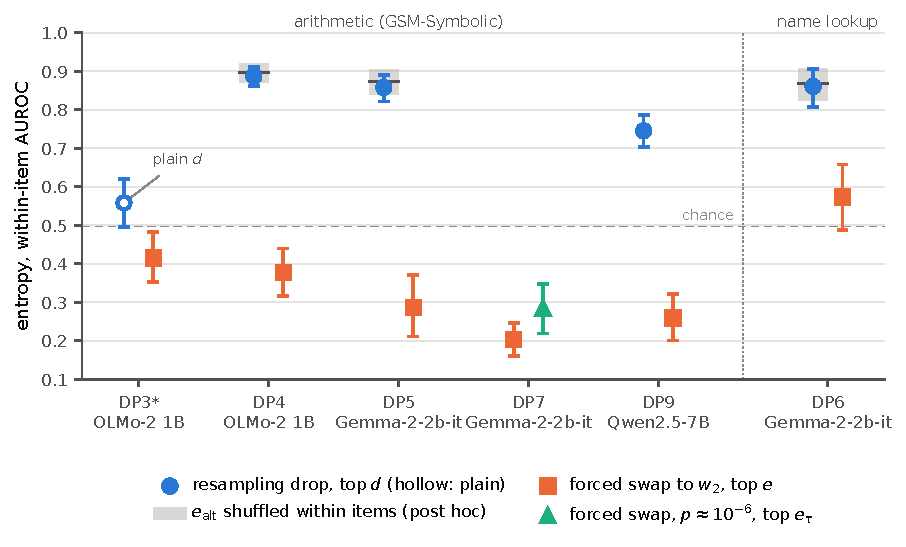
\includegraphics{../figures/fig2_reversal.pdf}
\caption{Entropy's within-item AUROC for the top 15\% of positions under each definition (Table 2). *DP3: comparing either side with 0.5 was post hoc; DP3 is where the anti-alignment was first
separated from chance. Blue circles: resampling drop (hollow: plain estimate of \(d\), DP3; filled: stratified \(d_{s}\)). Grey bands: the same AUROC when each item's \(e_{\mathrm{alt}}\) is shuffled
across its positions while 1 − \(p_1\) is kept (post hoc, R1; band = 95\% range of 2,000 shuffles, line = mean; R1 predates DP9, so DP9 has no band). Orange squares: forced swap to the runner-up (top
\(e\)). Green triangle: forced swap to a token of probability about \(10^{-6}\) (top \(e_{\tau}\), DP7, matched positions). DP9 is Qwen2.5-7B-Instruct (§3.6). Vertical bars are 95\% bootstrap
intervals (template-level; item-level in DP6); the dashed line is chance.}
\end{figure}

\begin{itemize}
\tightlist
\item
  On arithmetic (DP3--DP5, DP7, DP9) every forced-swap interval lies below 0.5. In the name-lookup check (DP6) the forced-swap side is indistinguishable from 0.5, while the resampling side is far
  above it.
\item
  The anti-alignment was first separated from chance in DP3 (post hoc: 0.415 against a within-item permutation null of mean 0.500, two-sided p = 0.0025); DP3's registered control is discussed in
  Appendix B.
\end{itemize}

\textbf{Robustness (post hoc, R1, and pre-specified secondary analyses of DP7).}

\begin{itemize}
\tightlist
\item
  \emph{Threshold.} Labelling the top 5, 10, 20, 30 or 50\% instead of 15\% leaves every arithmetic point estimate (DP3--DP5, DP7) below 0.5, and the anti-alignment roughly grows as the cut tightens
  (DP5: 0.194 {[}0.115, 0.295{]} at 5\% and 0.403 {[}0.343, 0.465{]} at 50\%; DP7, top \(e_{\tau}\): 0.177 {[}0.105, 0.264{]} and 0.427 {[}0.375, 0.479{]}). The only interval that reaches 0.5 is DP3's
  at 50\% ({[}0.418, 0.504{]}).
\item
  \emph{No labels.} The mean within-item Spearman correlation between entropy and \(e\) is −0.092 {[}−0.148, −0.038{]} (DP3), −0.149 {[}−0.226, −0.067{]} (DP4) and −0.214 {[}−0.278, −0.150{]} (DP5),
  all outside within-item permutation nulls centred near 0; in DP7 it is −0.268 for \(e\) and −0.195 for \(e_{\tau}\) (permutation 95\% ranges about ±0.08).
\item
  \emph{Ties and unreadable answers.} Breaking ties at the cut at random, or counting unreadable continuations as unchanged or dropping them instead of counting them as changed, moves the AUROCs by
  about 0.03 at most; for the answer-format variants every arithmetic interval stays below 0.5. Unreadable answers are rare (0--3.5\% of continuations).
\item
  \emph{Reliability.} The labels are stable: in DP7 the split-half correlation of \(e\) is 0.854 and of \(e_{\tau}\) 0.876.
\item
  \emph{Headroom (post hoc, HR-1, plan frozen before computing).} A forced swap can raise the chance of a changed answer by at most 1 − \(q_{\mathrm{keep}}\), so if \(q_{\mathrm{keep}}\) rose with
  entropy within items, headroom alone could produce anti-alignment. It did not: within items, entropy and \(q_{\mathrm{keep}}\) were essentially uncorrelated (mean Spearman between −0.011 and +0.068,
  every interval including 0; DP4, DP5, DP7, DP9). Dividing \(e\) by 1 − \(q_{\mathrm{keep}}\), or keeping only positions with \(q_{\mathrm{keep}}\) ≤ 0.5, left every interval below 0.5 (DP4 0.348 and
  0.335, DP5 0.234 and 0.280, DP7 0.189 and 0.149, DP9 0.260 and 0.238; upper ends 0.418 at most), so the anti-alignment is not a headroom effect.
\end{itemize}

\textbf{Pre-specified secondary analyses: solved versus unsolved items.} The anti-alignment is strongest on items the model solves. Entropy's AUROC for top \(e\) on solved versus unsolved items is
0.343 {[}0.211, 0.497{]} versus 0.456 {[}0.401, 0.508{]} (DP3), 0.320 {[}0.238, 0.396{]} versus 0.442 {[}0.353, 0.539{]} (DP4), 0.151 {[}0.098, 0.214{]} versus 0.420 {[}0.303, 0.547{]} (DP5), 0.139
{[}0.098, 0.183{]} versus 0.289 {[}0.224, 0.346{]} (DP7) and 0.247 {[}0.180, 0.318{]} versus 0.337 {[}0.286, 0.399{]} (DP9, where only 5 items were unsolved). On unsolved items the interval includes
0.5 in DP3 (only just), DP4 and DP5, but not in DP7 or DP9. One reason for the gap is mechanical: \(e \le 1-q_{\mathrm{keep}}\), and \(q_{\mathrm{keep}}\) tends to be high on unsolved items (on DP1's
records, mean 0.64 versus 0.15 on solved items; post hoc).

\hypertarget{the-resampling-sides-alignment-largely-follows-from-the-definition}{%
\subsection{The resampling side's alignment largely follows from the definition}\label{the-resampling-sides-alignment-largely-follows-from-the-definition}}

\textbf{The weighting test (pre-registered).} By the identity, \(d_{s} = (1-p_1) \cdot e_{\mathrm{alt}}\). The weighting tests compare entropy's AUROC for top \(d_{s}\) with that for top
\(e_{\mathrm{alt}}\) at the same positions (Table 3, Figure 3).

\begin{longtable}[]{@{}
  >{\raggedright\arraybackslash}p{(\columnwidth - 8\tabcolsep) * \real{0.2425}}
  >{\raggedright\arraybackslash}p{(\columnwidth - 8\tabcolsep) * \real{0.1746}}
  >{\raggedright\arraybackslash}p{(\columnwidth - 8\tabcolsep) * \real{0.1843}}
  >{\raggedright\arraybackslash}p{(\columnwidth - 8\tabcolsep) * \real{0.1843}}
  >{\raggedright\arraybackslash}p{(\columnwidth - 8\tabcolsep) * \real{0.1843}}@{}}
\caption{The weighting tests (pre-registered) and the weight-only baseline (post hoc; R1 predates DP9).}\tabularnewline
\toprule\noalign{}
\begin{minipage}[b]{\linewidth}\raggedright
\end{minipage} & \begin{minipage}[b]{\linewidth}\raggedright
DP4 OLMo-2 1B
\end{minipage} & \begin{minipage}[b]{\linewidth}\raggedright
DP5 Gemma-2-2b-it
\end{minipage} & \begin{minipage}[b]{\linewidth}\raggedright
DP9 Qwen2.5-7B-Instruct
\end{minipage} & \begin{minipage}[b]{\linewidth}\raggedright
DP6 Gemma-2-2b-it (name lookup)
\end{minipage} \\
\midrule\noalign{}
\endfirsthead
\toprule\noalign{}
\begin{minipage}[b]{\linewidth}\raggedright
\end{minipage} & \begin{minipage}[b]{\linewidth}\raggedright
DP4 OLMo-2 1B
\end{minipage} & \begin{minipage}[b]{\linewidth}\raggedright
DP5 Gemma-2-2b-it
\end{minipage} & \begin{minipage}[b]{\linewidth}\raggedright
DP9 Qwen2.5-7B-Instruct
\end{minipage} & \begin{minipage}[b]{\linewidth}\raggedright
DP6 Gemma-2-2b-it (name lookup)
\end{minipage} \\
\midrule\noalign{}
\endhead
\bottomrule\noalign{}
\endlastfoot
Entropy AUROC, top \(d_{s}\) & 0.887 & 0.858 & 0.745 & 0.860 \\
Entropy AUROC, top \(e_{\mathrm{alt}}\) & 0.352 & 0.301 & 0.239 & 0.505 \\
Difference & +0.535 {[}0.465, 0.604{]} & +0.557 {[}0.465, 0.649{]} & +0.506 {[}0.438, 0.570{]} & +0.356 {[}0.260, 0.447{]} \\
Registered outcome & confirmed & confirmed & confirmed & confirmed \\
Estimator check, mean(\(d_{s} - d_{\mathrm{plain}}\)) & 0.00001 {[}−0.0055, +0.0056{]} & −0.0027 {[}−0.0121, +0.0071{]} & −0.0002 {[}−0.0039, +0.0037{]} & −0.0013 {[}−0.0138, +0.0112{]} \\
Weight-only baseline, mean {[}95\% range{]} (post hoc, R1) & 0.897 {[}0.872, 0.920{]} & 0.873 {[}0.840, 0.904{]} & not computed & 0.868 {[}0.823, 0.906{]} \\
\end{longtable}

Multiplying by \((1-p_1)\) turns an anti-aligned quantity (\(e_{\mathrm{alt}}\)) into a strongly aligned one (\(d_{s}\)). In DP3, which used the plain estimator, the difference (top \(d\) minus top
\(e\)) was +0.143 {[}0.035, 0.245{]}, in the predicted direction but short of the registered margin of 0.05 (undecided under its rule); its labels were too noisy (see \emph{Measurement}, below).

\textbf{How much is built in.} A positive result was expected in advance. A power simulation written while DP4 was running, before any results were seen (Appendix A), confirmed the weighting in 60 of
60 runs at every assumed relation between entropy and effect size, including none at all, where the top-\(d_{s}\) AUROC was still about 0.85. The reason is that 1 − \(p_1\) ranges over several orders
of magnitude across positions, while \(e_{\mathrm{alt}}\) lies between −1 and 1, so the ranking by \(d_{s}\) is set mostly by 1 − \(p_1\). R1 measured this on the real records: keeping each position's
1 − \(p_1\) and entropy and shuffling \(e_{\mathrm{alt}}\) within items gives the AUROCs in the last row of Table 3, and the observed values lie inside those ranges in all three experiments where it
was computed (in 77\%, 83\% and 64\% of shuffles the shuffled value was at least as high as the observed one). Ranking by 1 − \(p_1\) alone gives 0.990, 0.998 and 0.967. In DP6, \(e_{\mathrm{alt}}\)
was at chance (0.505), yet \(d_{s}\) reached 0.860. The resampling side's alignment with entropy is therefore indistinguishable from what the weight produces with effects unrelated to position; the
shuffles vary by 0.05--0.08, so a small contribution of \(e_{\mathrm{alt}}\) is not excluded. We read the weighting outcomes as confirming that the decomposition behaves as derived, not as evidence
for a mechanism.

\begin{figure}
\centering
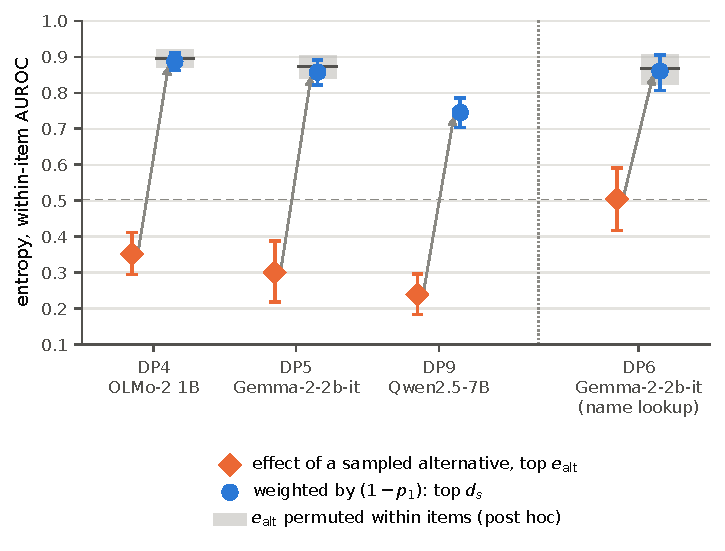
\includegraphics{../figures/fig3_weighting.pdf}
\caption{The weighting step, at the same positions. Orange diamonds: entropy's within-item AUROC for the top 15\% of positions by \(e_{\mathrm{alt}} = q_{\mathrm{alt}} - q_{\mathrm{keep}}\), the
effect of replacing \(w_1\) by a sampled alternative. Blue circles: the same for \(d_{s} = (1-p_1) \cdot e_{\mathrm{alt}}\). The arrows mark the multiplication by \((1-p_1)\). Grey bands: the
top-\(d_{s}\) AUROC with \(e_{\mathrm{alt}}\) shuffled within items and 1 − \(p_1\) kept (post hoc, R1; 95\% range of 2,000 shuffles, line = mean; not computed for DP9, Qwen2.5-7B-Instruct). Bars are
95\% bootstrap intervals (template-level; item-level in DP6); the dashed line is chance. In DP6, \(e_{\mathrm{alt}}\) was not anti-aligned to begin with, so the weighting raised the AUROC from chance
rather than reversing it.}
\end{figure}

\textbf{Measurement: the stratified drop makes resampling labels usable.} With the plain estimator, resampling labels are very noisy at feasible sample sizes: the split-half correlation of the
estimated \(d\) (16 versus 16 samples) was −0.02 in DP3. At the same positions and sampling cost, stratifying on the first token raised it from −0.02 to 0.43 (DP4) and from 0.04 to 0.43 (DP5), without
changing the estimand (the estimator checks in Table 3 stay within ±0.02; pre-specified secondary analyses). The agreement of the top-15\% labels between halves rose less (DP4: 0.765 → 0.834; DP5,
same positions: 0.783 → 0.847). The plain estimator's standard deviation does not shrink at confident positions, while the true drop is bounded by 1 − \(p_1\) and is near zero there (Appendix A). In
Qwen2.5-7B-Instruct (DP9) \(d_{s}\) was much less reliable (split-half 0.14 over all positions, against 0.68 in DP5), though still above the plain estimate on its free positions (−0.04); in that very
confident model \(d_{s}\) is close to zero at most positions (§3.6).

\hypertarget{what-drives-the-anti-alignment-confident-digit-tokens-not-only-the-size-of-the-swap}{%
\subsection{What drives the anti-alignment: confident digit tokens, not only the size of the swap}\label{what-drives-the-anti-alignment-confident-digit-tokens-not-only-the-size-of-the-swap}}

\textbf{Digits (pre-registered).}

\begin{itemize}
\tightlist
\item
  DP3 (OLMo-2 1B): forced swaps change the answer at 58\% of digit positions versus 29\% of others (+0.30 {[}0.22, 0.39{]}); entropy's AUROC for forced forks rises from 0.481 to 0.572 without digits
  (+0.091 {[}0.037, 0.155{]}); confirmed.
\item
  DP5 (Gemma-2-2b-it), the first registered test that digits drive the anti-alignment (motivated by a secondary analysis of DP4 without a decision rule, read post hoc: OLMo's top-e AUROC was 0.378
  overall and 0.464 without digits). Digit positions are 20\% of positions but about 64\% of the top-e positions; the rate of top-e positions is 0.473 among digit positions versus 0.067 elsewhere
  (+0.406 {[}0.314, 0.505{]}). Removing digits moves entropy's top-e AUROC from 0.286 to 0.452 (+0.166 {[}0.058, 0.285{]}); confirmed. Digit tokens are confident: mean entropy 0.08 versus 0.28
  elsewhere.
\item
  Without digits, DP5's interval {[}0.327, 0.583{]} includes 0.5, and only 17 items have both classes there. Restricted post hoc to those 17 items for both values, the difference is +0.099 {[}0.027,
  0.177{]} (R1). We claim that digit tokens carry a substantial part of the anti-alignment, not all of it.
\item
  DP9 (Qwen2.5-7B-Instruct) replicated DP5's test with the same rule. Digit positions are 19\% of positions but about 60\% of the top-e positions (top-e rate 0.482 versus 0.073; +0.408 {[}0.331,
  0.487{]}). Removing digits moves the top-e AUROC from 0.259 to 0.485 {[}0.363, 0.597{]} (+0.226 {[}0.133, 0.320{]}, 18 items with both classes); confirmed. Digit tokens are even more confident
  there: mean entropy 0.016 versus 0.174 elsewhere.
\end{itemize}

\textbf{Entropy and swap size are entangled in observational data.} Entropy and the runner-up's probability \(p_2\) rank positions almost identically (Spearman 0.985, 0.976, 0.988 and 0.937 in
DP3--DP6). ``Large forced-swap effects sit at low-entropy positions'' is therefore also ``they sit where the runner-up is improbable'', where a forced swap is a large, off-policy perturbation
(cf.~Macar et al., 2026). Two post hoc analyses (R1) bear on this without separating it:

\begin{itemize}
\tightlist
\item
  Holding \(p_2\) fixed (strata of item × \(p_2\) quintile), digit positions are still much more likely to be top \(e\): Mantel--Haenszel odds ratio 5.12 {[}3.26, 8.65{]} (DP3), 6.15 {[}3.54, 12.45{]}
  (DP4) and 23.19 {[}10.50, 112.04{]} (DP5); a label-permutation control was centred at 1 in each (medians 0.97--1.01).
\item
  Among non-digit positions, the share of top-e positions barely changes across \(p_2\) tertiles (DP3 13/9/12\%, DP4 14/9/9\%, DP5 7/6/7\%, from the most to the least confident third; descriptive). At
  digit positions, effects are largest when the runner-up is another digit (top-e rate 48--58\%) and small when it is whitespace (0--9\%).
\end{itemize}

\textbf{The probability-matched swap (DP7, pre-registered).} To separate confidence from swap size, DP7 forced, at every position, a second swap to the token \(w_{\tau}\) whose probability is closest
to \(\tau = 10^{-6}\), so that the swapped-in token is about equally improbable everywhere. 95.3\% of positions were matched (811 of 851; \(\log_{10}\) \(p\)(\(w_{\tau}\)) between −6.20 and −5.81 for
90\% of them). If the anti-alignment came from swapping in more improbable tokens at confident positions, it should vanish for \(e_{\tau}\); if it came from the positions themselves, it should remain
(Table 4).

\begin{longtable}[]{@{}
  >{\raggedright\arraybackslash}p{(\columnwidth - 6\tabcolsep) * \real{0.3492}}
  >{\raggedright\arraybackslash}p{(\columnwidth - 6\tabcolsep) * \real{0.2037}}
  >{\raggedright\arraybackslash}p{(\columnwidth - 6\tabcolsep) * \real{0.1164}}
  >{\raggedright\arraybackslash}p{(\columnwidth - 6\tabcolsep) * \real{0.3007}}@{}}
\caption{The pre-registered tests of the probability-matched swap (full rules in Appendix B).}\tabularnewline
\toprule\noalign{}
\begin{minipage}[b]{\linewidth}\raggedright
DP7 test (matched positions)
\end{minipage} & \begin{minipage}[b]{\linewidth}\raggedright
Value {[}95\% CI{]}
\end{minipage} & \begin{minipage}[b]{\linewidth}\raggedright
Rule
\end{minipage} & \begin{minipage}[b]{\linewidth}\raggedright
Outcome
\end{minipage} \\
\midrule\noalign{}
\endfirsthead
\toprule\noalign{}
\begin{minipage}[b]{\linewidth}\raggedright
DP7 test (matched positions)
\end{minipage} & \begin{minipage}[b]{\linewidth}\raggedright
Value {[}95\% CI{]}
\end{minipage} & \begin{minipage}[b]{\linewidth}\raggedright
Rule
\end{minipage} & \begin{minipage}[b]{\linewidth}\raggedright
Outcome
\end{minipage} \\
\midrule\noalign{}
\endhead
\bottomrule\noalign{}
\endlastfoot
Entropy AUROC, top \(e\) (runner-up swap; prerequisite) & 0.203 {[}0.160, 0.246{]} & upper \textless{} 0.50 & confirmed (prerequisite met) \\
Entropy AUROC, top \(e_{\tau}\) (probability-matched swap) & 0.283 {[}0.219, 0.348{]} & upper \textless{} 0.50 & confirmed (persists) \\
Odds ratio of top \(e_{\tau}\) for digit positions, strata item × entropy quintile & 48.8 {[}22.9, 231.7{]} & lower \textgreater{} 1 & confirmed (digits more fragile) \\
\end{longtable}

\begin{itemize}
\tightlist
\item
  The anti-alignment persists when the swapped-in token's probability is held fixed. Large effects of a matched swap still sit at confident positions (Figure 4a): the mean \(e_{\tau}\) is 0.260 in the
  most confident entropy tertile and 0.075 and 0.072 in the other two.
\item
  At equal entropy, digit positions are far more fragile. They are 19\% of matched positions and 72\% of the top-\(e_{\tau}\) positions (top-\(e_{\tau}\) rate 0.572 versus 0.052). The
  label-permutation control was centred at 1.04.
\item
  Swap size is not irrelevant. In the most uncertain tertile, \(e_{\tau}\) exceeds \(e\) by 0.056 on average (an improbable token does break uncertain positions more often than the runner-up), and the
  AUROC for top \(e_{\tau}\) (0.283) is somewhat closer to 0.5 than that for top \(e\) (0.203). This difference was not a registered comparison and has no interval; the two intervals overlap.
\item
  What is swapped in still differs between positions. At digit positions, 96 of 152 matched tokens \(w_{\tau}\) were themselves digit-bearing (Figure 4b), so a matched swap there often replaces one
  number by another. Inserting a token that is neither digit-bearing nor whitespace at a digit position was also fragile (top-\(e_{\tau}\) rate 0.385, 39 positions), against 0.055 for such tokens at
  non-digit positions; we cannot apportion the effect between the position and the kind of token swapped in.
\item
  \emph{Rank of the matched token (post hoc, RK-1, plan frozen before computing).} DP7 fixed the probability of \(w_{\tau}\), not its rank. We recomputed DP7's base paths teacher-forced with DP7's own
  code. The greedy token, \(w_{\tau}\) and its probability (within 1\%) were reproduced at all 6,651 steps and 851 analysed positions. The rank did vary, but \(w_{\tau}\) ranked nearer the top where
  the model was confident: median rank 4, 12 and 27 from the most to the least confident entropy tertile (within-item Spearman between entropy and log rank 0.83 {[}0.81, 0.86{]}), and higher-ranked
  \(w_{\tau}\) went with larger \(e_{\tau}\) (Spearman between log rank and \(e_{\tau}\) −0.16 {[}−0.24, −0.07{]}). So where effects were large, the inserted token was not further from the model's
  choices by rank. Split at the median rank (11), the anti-alignment holds where \(w_{\tau}\) ranks 11 or better (0.299 {[}0.241, 0.360{]}, 31 items with both classes). Where it ranks lower, it is
  undecided (0.431 {[}0.324, 0.536{]}; only 33 top-\(e_{\tau}\) positions in 16 items), so we cannot exclude that rank contributes part of it. Because rank and entropy are so closely linked, that half
  consists mostly of uncertain positions and covers only part of the entropy range. Holding item × log-rank quintile fixed, digit positions remain far more fragile (odds ratio 66.8 {[}33.2, 262.0{]},
  one bootstrap resample undefined; permutation control centred at 1.01).
\item
  The 40 unmatched positions were the most confident ones (median entropy \(4.5\times 10^{-5}\) versus \(2.4\times 10^{-2}\)), where no token lies near \(10^{-6}\). Excluding them, as registered, is
  expected to work against the anti-alignment.
\item
  In Qwen2.5-7B-Instruct this control was made descriptive before the run, because a smoke run had matched only 47\% of positions; in the run only 16\% of digit positions were matched (§3.6). DP7's
  conclusion rests on Gemma alone.
\end{itemize}

\begin{figure}
\centering
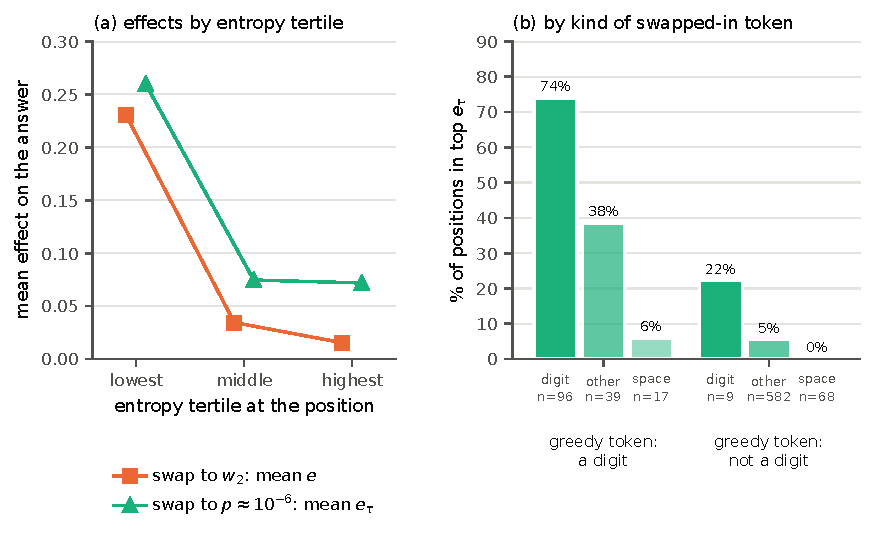
\includegraphics{../figures/fig4_matched_swap.pdf}
\caption{The probability-matched swap (DP7, matched positions; pre-specified secondary analyses). (a) Mean effect of forcing the runner-up (\(e\), orange squares) and of forcing a token of probability
about \(10^{-6}\) (\(e_{\tau}\), green triangles), by entropy tertile of the position (270--271 positions each). (b) Share of positions in the top 15\% of \(e_{\tau}\), by whether the greedy token is
a digit and by the kind of token swapped in (digit-bearing, other, whitespace); n is the number of positions.}
\end{figure}

\textbf{Other features (exploratory, EX-1, Appendix H).} A sweep of 20 features of a position, frozen before computing and without correction for multiple comparisons, found nothing beyond confidence
and digits. The nine features that met a mechanical candidate rule in DP4 and DP5 and then held in DP7 and DP9 all measure confidence or digits. At non-digit positions, no feature pointed the same way
across the experiments, although with 16--18 items with both classes in three of them this absence has little power.

\textbf{Readout (post hoc, R1).} Digits in the last computation line feed the final-answer line directly, so part of the fragility could be readout rather than computation (cf.~Garcia, 2026). Removing
the final-answer line, the last non-empty line before it and every number equal to the answer (labels kept) leaves Gemma's anti-alignment unchanged (DP5: 0.286 → 0.274 {[}0.192, 0.356{]}; R1 reading
``anti-alignment survives readout''). For OLMo the result is undecided (DP3: 0.415 → 0.464 {[}0.386, 0.547{]}; DP4: 0.378 → 0.433 {[}0.353, 0.517{]}): the shifts are within what removing the same
number of random positions produces, and most of them come from 8 (DP3) and 16 (DP4) items whose positions all lie in the removed lines and which drop out. Removing only the numbers equal to the
answer leaves all three intervals below 0.5.

\hypertarget{a-boundary-name-lookup-dp6}{%
\subsection{A boundary: name lookup (DP6)}\label{a-boundary-name-lookup-dp6}}

\textbf{Design (pre-registered).}

\begin{itemize}
\tightlist
\item
  A synthetic task with name-valued answers (English, fictional names). Each item has its own roster of eight people and twelve relation records. The model identifies a starting person, follows a
  fixed number of records (``hops'') and answers with a full name.
\item
  Name positions (tokens overlapping a roster name) play the role of digit positions.
\item
  The number of hops was set per model by a separate calibration run: 20 fresh items per hop count (one to three), greedy answers only, no fork quantities. The rule picked the hop count with accuracy
  closest to 0.55 within 0.30--0.80 (else within 0.20--0.90; ties to more hops). The answer-line reading was amended before any model was run.
\item
  Fork quantities, sampling and analysis are as in DP5; intervals use an item-level bootstrap. Table 5 compares the two tasks.
\end{itemize}

\textbf{Models run.}

\begin{itemize}
\tightlist
\item
  OLMo-2 1B could not perform the task: calibration accuracy 0.15, 0.05 and 0.10 at one to three hops, near chance for eight names and below the pre-registered guard of 0.20. It therefore had no main
  run.
\item
  Gemma-2-2b-it: calibration accuracy 0.50, 0.85 and 0.45 at one to three hops (we had predicted two hops), so the rule chose one hop. With 20 items per hop count these accuracies have standard errors
  of about 0.08--0.11, so the choice of one hop is partly chance. Main run: 40 items, 388 positions. Base accuracy 0.725; estimator check −0.0013 {[}−0.0138, +0.0112{]}; replay audit: 0 diverged
  items.
\end{itemize}

\begin{longtable}[]{@{}
  >{\raggedright\arraybackslash}p{(\columnwidth - 4\tabcolsep) * \real{0.3880}}
  >{\raggedright\arraybackslash}p{(\columnwidth - 4\tabcolsep) * \real{0.2910}}
  >{\raggedright\arraybackslash}p{(\columnwidth - 4\tabcolsep) * \real{0.2910}}@{}}
\caption{Arithmetic (DP5) and name lookup (DP6) compared, both on Gemma-2-2b-it.}\tabularnewline
\toprule\noalign{}
\begin{minipage}[b]{\linewidth}\raggedright
\end{minipage} & \begin{minipage}[b]{\linewidth}\raggedright
DP5 (arithmetic)
\end{minipage} & \begin{minipage}[b]{\linewidth}\raggedright
DP6 (name lookup)
\end{minipage} \\
\midrule\noalign{}
\endfirsthead
\toprule\noalign{}
\begin{minipage}[b]{\linewidth}\raggedright
\end{minipage} & \begin{minipage}[b]{\linewidth}\raggedright
DP5 (arithmetic)
\end{minipage} & \begin{minipage}[b]{\linewidth}\raggedright
DP6 (name lookup)
\end{minipage} \\
\midrule\noalign{}
\endhead
\bottomrule\noalign{}
\endlastfoot
Entropy AUROC, top \(d_{s}\) − top \(e_{\mathrm{alt}}\) & +0.557 {[}0.465, 0.649{]} & +0.356 {[}0.260, 0.447{]} \\
Entropy AUROC, top \(e_{\mathrm{alt}}\) & 0.301 {[}0.218, 0.389{]} & 0.505 {[}0.417, 0.590{]} \\
Entropy AUROC, top \(e\) & 0.286 {[}0.211, 0.370{]} & 0.574 {[}0.488, 0.658{]} \\
Registered outcome for top \(e\) & anti-alignment confirmed & not replicated \\
Entropy AUROC, top \(e\), digit / name positions removed & 0.452 & 0.591 \\
Difference (removed − all) & +0.166 {[}0.058, 0.285{]} (confirmed) & +0.018 {[}−0.068, +0.109{]} (undecided) \\
Mean entropy, digit / name positions vs others & 0.08 vs 0.28 & 0.13 vs 0.69 \\
Share of top-e positions that are digit / name positions (share of all positions) & 64\% (20\%) & 28\% (24\%) \\
\end{longtable}

\begin{figure}
\centering
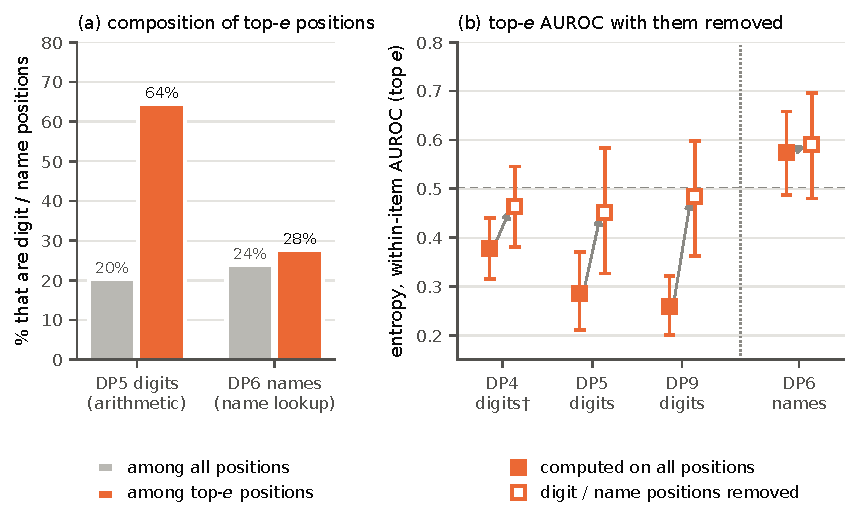
\includegraphics{../figures/fig5_digits_names.pdf}
\caption{Digit tokens (arithmetic) versus name tokens (name lookup). (a) Grey: share of analysed positions that are digit positions (DP5, 184 of 905) or name positions (DP6, 93 of 388). Orange: their
share among the top-e positions (DP5, 87 of 135; DP6, 16 of 58). This re-expresses the registered comparison of top-e rates: 0.473 at digit positions versus 0.067 elsewhere in DP5, and 0.172 at name
positions versus 0.142 elsewhere in DP6 (read descriptively). (b) Entropy's within-item AUROC for top \(e\) on all positions (filled) and with digit or name positions removed (hollow), with 95\%
bootstrap intervals (template-level; item-level in DP6); DP9 is Qwen2.5-7B-Instruct (§3.3, §3.6). The top-e labels are those of the full analysis and are not re-ranked after removal. †DP4: a secondary
analysis listed in the DP4 gate without a decision rule; reading it as a digit effect came after the run and motivated the DP5 hypothesis (§3.3).}
\end{figure}

\begin{itemize}
\tightlist
\item
  The weighting replicated, as expected by construction (§3.2). Here nothing flipped: \(e_{\mathrm{alt}}\) showed no anti-alignment (0.505 {[}0.417, 0.590{]}), unlike in DP4 (0.352) and DP5 (0.301).
\item
  The anti-alignment did not replicate. The value lies inside the 95\% range of a within-item permutation control (2,000 permutations), {[}0.404, 0.595{]}. The label-free rank correlation is also null
  (0.005 {[}−0.102, 0.103{]}; post hoc).
\item
  Labels were noisier than in DP5 (split-half correlation of \(e\) 0.56 versus 0.85). This pulls the AUROC towards 0.5, so a weak anti-alignment is not excluded. Post hoc, labelling only the top 5\%
  or 10\% gives AUROCs \emph{above} 0.5 (0.637 {[}0.562, 0.711{]} and 0.647 {[}0.565, 0.731{]}; 15 and 25 items with both classes).
\item
  With no anti-alignment to explain, the registered test of whether name tokens drive it was undecided. Holding \(p_2\) fixed, name positions were not separated from others (odds ratio 2.67 {[}0.87,
  18.28{]}; post hoc).
\item
  Secondary: even on correctly solved items, no anti-alignment was seen (0.547 {[}0.426, 0.659{]}; DP5: 0.151).
\item
  Our predictions were wrong: we had expected anti-alignment (0.35--0.45) driven by name tokens.
\end{itemize}

\textbf{Post hoc.} Name tokens were confident, like digits, but large forced-swap effects were not noticeably concentrated on them (Figure 5): the rate of top-e positions was 0.17 at name positions
versus 0.14 elsewhere (difference +0.030 {[}−0.037, +0.100{]}; this is the registered condition of the name test, read here descriptively). One reading, consistent with this but untested, is that the
anti-alignment needs tokens that are both confident and answer-breaking when swapped: in arithmetic, digits are such tokens; in this lookup task, names were not disproportionately so. DP6's runner-ups
were also less improbable: the most confident third of positions had \(p_2\) below \(2.4\times 10^{-3}\), against \(5.0\times 10^{-5}\) in DP4 and \(2.2\times 10^{-4}\) in DP5. DP7 argues against a
pure swap-size explanation of the arithmetic result, but DP6 itself did not vary swap size.

\textbf{Scope.} One model, one synthetic task, one hop; the change of task is confounded with chain depth. How the two-model gate was applied after OLMo-2 1B dropped out (a choice made after seeing
the result) is recorded in Appendix B.

\hypertarget{rare-alternatives-large-effects-when-they-occur-little-contribution-to-how-answers-vary}{%
\subsection{Rare alternatives: large effects when they occur, little contribution to how answers vary}\label{rare-alternatives-large-effects-when-they-occur-little-contribution-to-how-answers-vary}}

The forced-swap effects of §3.3 sit at confident positions, where an alternative is rarely sampled. Two questions follow. Is an alternative that the model itself samples as damaging as one that we
force? And how much do such positions contribute to how the answer varies under ordinary sampling? We write r = 1 − \(p_1\) for the chance that any alternative is sampled at a position.

\textbf{Exploratory origin (DP8-X, post hoc).} We rebuilt the position tables of DP4, DP5 and DP7 from their records with each experiment's own code (each experiment's analysis was reproduced to
within \(10^{-9}\) of the recorded result), split positions into six bands of r and compared the effects, with views fixed before looking. Four patterns appeared. In every band \(e_{\mathrm{alt}}\)
and \(e\) were about equal. The largest effects sat in the rarest band at digit positions. Positions with r ≤ 0.05 contributed 4.4\% (DP4, OLMo-2 1B) and 3.7\% (DP5, Gemma-2-2b-it) of the summed drop
\(d_{s}\). In DP7, the \(10^{-6}\) token broke slightly more often than the runner-up in every band. DP8 tested these four patterns on new items.

\textbf{Design (DP8, pre-registered).} Gemma-2-2b-it, 40 new GSM-Symbolic items (all earlier items and the candidates of the closed-model study of Appendix D excluded), positions every 8th token. At
each position four branches of 32 continuations: keep, swap (\(w_2\)), alt (the first token sampled with \(w_1\) removed, as in DP4--DP6, with the id of the sampled token recorded) and the
probability-matched swap of DP7. Bands of r have edges \(10^{-4}\), \(10^{-3}\), \(10^{-2}\), 0.05 and 0.2. Base accuracy was 0.650; 38 items had a readable base answer (826 positions); 96.6\% of
positions were matched; the replay audit (5 items × 3 points, all four branches, also the first token of alt and the choice of \(w_{\tau}\)) found 0 diverged items; Table 6 gives the tests.

\begin{longtable}[]{@{}
  >{\raggedright\arraybackslash}p{(\columnwidth - 6\tabcolsep) * \real{0.4074}}
  >{\raggedright\arraybackslash}p{(\columnwidth - 6\tabcolsep) * \real{0.1940}}
  >{\raggedright\arraybackslash}p{(\columnwidth - 6\tabcolsep) * \real{0.1649}}
  >{\raggedright\arraybackslash}p{(\columnwidth - 6\tabcolsep) * \real{0.2037}}@{}}
\caption{The pre-registered tests of DP8 (full rules in Appendix B). All four came out as predicted.}\tabularnewline
\toprule\noalign{}
\begin{minipage}[b]{\linewidth}\raggedright
DP8 test
\end{minipage} & \begin{minipage}[b]{\linewidth}\raggedright
Value {[}95\% CI{]}
\end{minipage} & \begin{minipage}[b]{\linewidth}\raggedright
Rule
\end{minipage} & \begin{minipage}[b]{\linewidth}\raggedright
Outcome
\end{minipage} \\
\midrule\noalign{}
\endfirsthead
\toprule\noalign{}
\begin{minipage}[b]{\linewidth}\raggedright
DP8 test
\end{minipage} & \begin{minipage}[b]{\linewidth}\raggedright
Value {[}95\% CI{]}
\end{minipage} & \begin{minipage}[b]{\linewidth}\raggedright
Rule
\end{minipage} & \begin{minipage}[b]{\linewidth}\raggedright
Outcome
\end{minipage} \\
\midrule\noalign{}
\endhead
\bottomrule\noalign{}
\endlastfoot
Natural alternative versus runner-up: mean of \(e - e_{\mathrm{alt}}\) (all positions) & −0.004 {[}−0.010, +0.003{]} & interval within ±0.03 → like & confirmed (alike) \\
Rarer alternatives hurt more: within-item Spearman of r and \(e_{\mathrm{alt}}\) & −0.340 {[}−0.405, −0.276{]} & upper \textless{} 0 & confirmed (rarer hurts more) \\
Share of the summed drop \(d_{s}\) from positions with r ≤ 0.05 & −0.002 {[}−0.043, +0.026{]} & upper \textless{} 0.10 & confirmed (little) \\
Probability-matched swap versus runner-up: mean of \(e_{\tau} - e\) (matched positions) & +0.030 {[}+0.016, +0.044{]} & lower \textgreater{} 0 & confirmed (\(10^{-6}\) token hurts more) \\
\end{longtable}

\begin{figure}
\centering
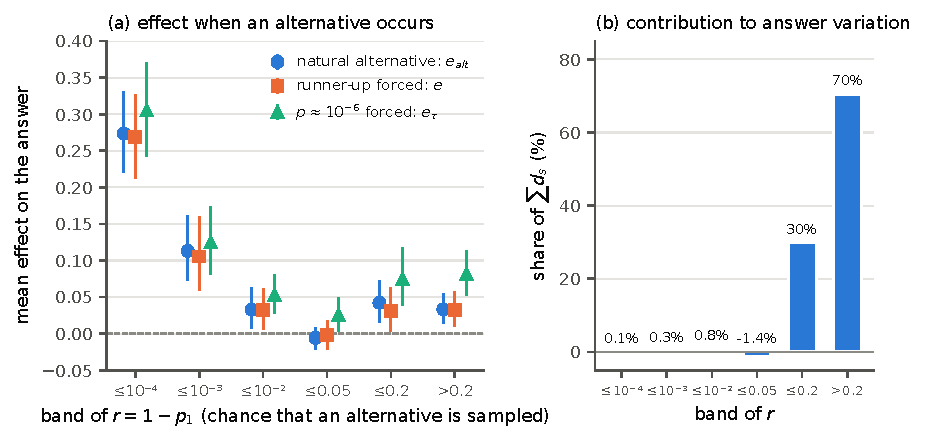
\includegraphics{../figures/fig6_rarity.pdf}
\caption{Rare alternatives (DP8, Gemma-2-2b-it, 826 positions). (a) Mean effect on the answer of the three alternatives at a position, by band of r = 1 − \(p_1\) (labels give each band's upper edge):
an alternative sampled from the model's distribution with the greedy token excluded (\(e_{\mathrm{alt}}\), blue circles), the runner-up forced (\(e\), orange squares) and a token of probability about
\(10^{-6}\) forced (\(e_{\tau}\), green triangles; matched positions). Bars are 95\% bootstrap intervals over items. (b) Share of the summed stratified drop \(d_{s}\) = r·\(e_{\mathrm{alt}}\) that
comes from each band (pre-specified secondary analysis).}
\end{figure}

\begin{itemize}
\tightlist
\item
  \textbf{An alternative the model samples is about as damaging as a forced one, and most damaging where it is rarest.} In the rarest band (r ≤ \(10^{-4}\); 225 positions, 56\% of them digits) the
  three effects were 0.273, 0.269 and 0.305 (\(e_{\tau}\) on its 201 matched positions); \(e - e_{\mathrm{alt}}\) there was −0.005 {[}−0.021, +0.012{]}, and at digit positions of all bands −0.013
  {[}−0.034, +0.007{]} (pre-specified secondary analyses; the latter is not within ±0.03). In the rarest band at digit positions \(e_{\mathrm{alt}}\) was 0.485 {[}0.394, 0.588{]}. At non-digit
  positions \(e_{\mathrm{alt}}\) stayed between −0.006 and +0.031 in every band (pre-specified secondary analyses).
\item
  \textbf{Not only the runner-up.} The natural alternative was the runner-up in 56\% of draws in the rarest band and in 65--79\% in the others. Counting only draws whose first token was not \(w_2\),
  \(e_{\mathrm{alt}}\) was 0.304 {[}0.247, 0.366{]} in the rarest band (digits 0.530) and 0.119 in the next one: alternatives other than the runner-up were about as damaging. We had expected the
  rarest band's draws to be mostly the runner-up; they were a majority, but a smaller one than in any other band.
\item
  \textbf{Rare positions contribute almost nothing to how answers vary.} Positions with r \textgreater{} 0.2 carried 70\% of the summed drop and those with 0.05 \textless{} r ≤ 0.2 another 30\%; the
  four bands with r ≤ 0.05 together −0.2\% (Figure 6b). A large effect at a position where an alternative almost never occurs barely moves the answer distribution. The identity bounds each position's
  drop (\textbar{}\(d_{s}\)\textbar{} ≤ r), but the bound alone does not make the share small: the 113 positions of the band 0.01 \textless{} r ≤ 0.05 alone could together carry up to their Σr, which
  is at least 1.13 (113 × 0.01), against a total of 1.61.
\item
  \textbf{Swap size matters a little.} The \(10^{-6}\) token changed the answer slightly more often than the runner-up (+0.030); at non-digit positions the difference was positive in every band and
  its interval excluded 0 in three of the six; unreadable answers rose with it (up to 4.8\% of continuations).
\end{itemize}

Read together with §3.1--§3.3 (our interpretation; DP8 itself has no entropy test): the fragility of confident digits does not appear to be an artefact of forcing, since the model's own departures
from such tokens were at least about as damaging; but those departures are so rare that nearly all of the variation in sampled answers arises at positions where alternatives are common. This is
consistent with reading the anti-alignment of forced-swap effects with entropy and the alignment of the resampling drop with entropy as two views of the same positions: the largest effects sit where
alternatives are least likely. DP9 repeated DP8's first three tests in a larger model (§3.6).

\hypertarget{a-larger-model-of-a-third-family-dp9}{%
\subsection{A larger model of a third family (DP9)}\label{a-larger-model-of-a-third-family-dp9}}

Every result in §3.1--§3.5 came from models of 1.5B to 2.6B parameters. DP9 asks whether they hold in a model about three to five times larger, from another family.

\textbf{Design (pre-registered replication).} Qwen2.5-7B-Instruct (7.6B parameters), 40 new GSM-Symbolic items, positions every 8th token, and at each position the four branches of DP8 (keep, swap,
alt, the probability-matched swap), 32 continuations each, plus free at every third position for the estimator check. The questions, chosen after all earlier results had been seen, repeat DP5's three
tests and DP8's first three with their original rules, and add one: whether entropy's AUROC for top \(d_{s}\) exceeds 0.5 (in DP4--DP6 this value entered only the weighting test). Two choices were
fixed before freezing, after a smoke run on four hand-written problems:

\begin{itemize}
\tightlist
\item
  \emph{The probability-matched swap is described, not tested.} Only 47\% of the smoke run's positions had a token within ±0.5 decades of \(10^{-6}\) (Gemma: 95.3\% in DP7, 96.6\% in DP8); the
  unmatched ones were almost all at the most confident positions, so a test on matched positions would compare a biased half.
\item
  \emph{An information guard replaces the accuracy range} (a 7B model could exceed 0.90): outcomes would be withheld if too few positions or items carried information, and an unreadable test would be
  reported as ``not confirmed'', never as ``not replicated'' (thresholds in Appendix B).
\end{itemize}

\textbf{Run.} Base accuracy 0.85; 39 items had a readable base answer (1,324 positions, 247 of them digit positions). No guard was triggered, the estimator check passed (Table 3), and the replay audit
(5 items × 3 points, all branches drawn at each point, the first tokens of alt and free and the choice of \(w_{\tau}\)) found 0 diverged items. Every rule and value is in Appendix B (Table 8, DP9
rows).

\begin{itemize}
\tightlist
\item
  \textbf{Six of seven tests came out as predicted.} The anti-alignment (0.259 {[}0.200, 0.321{]}, Table 2), the weighting (+0.506 {[}0.438, 0.570{]}, Table 3), the digit concentration (+0.226
  {[}0.133, 0.320{]}, §3.3), the equivalence of natural and forced alternatives (\(e - e_{\mathrm{alt}}\) +0.001 {[}−0.004, +0.006{]}) and the rarity correlation (−0.319 {[}−0.382, −0.256{]})
  replicated, in the same direction and of similar size as in the smaller models. A within-item permutation control (2,000 permutations) gave top \(d_{s}\) a mean of 0.500 (95\% range {[}0.435,
  0.568{]}) and top \(e\) 0.501 ({[}0.442, 0.562{]}). On the 34 solved and the 5 unsolved items separately, the anti-alignment, the alignment with the drop and the rarity correlation kept their
  direction, and \(e - e_{\mathrm{alt}}\) stayed within ±0.03 (pre-specified secondary analyses).
\item
  \textbf{The alignment with the resampling drop was confirmed but weakly measured} (0.745 {[}0.703, 0.786{]}, lower than 0.86--0.89 in the smaller models). The model is far more confident: 59\% of
  positions had r ≤ \(10^{-4}\) (DP8: 27\%), so \(d_{s}\) is near zero at most positions. Its split-half correlation was only 0.14, and the top-15\% cut for \(d_{s}\) was \(2.9\times 10^{-7}\), so top
  \(d_{s}\) comes close to separating positions with any sampled drop from those with none.
\item
  \textbf{The contribution of rare positions was undecided:} 5.4\% {[}−0.9\%, +16.9\%{]} against a 10\% line (the gate had predicted ``little''). This is not evidence that rare positions contribute;
  the test could not separate the share from 10\%. Positions with r \textgreater{} 0.05 carried 94.6\% of Σ \(d_{s}\) (68\% from r \textgreater{} 0.2), as in Gemma; most of the rest came from the band
  0.01 \textless{} r ≤ 0.05 (4.1\%), where Gemma's share was about zero.
\item
  \textbf{Rarity, as in DP8.} The large effects sat in the rarest band at digit positions (\(e_{\mathrm{alt}}\) 0.300, against 0.485 in DP8), and non-digit positions stayed between 0.009 and 0.028 in
  every band. In the rarest band, where 65\% of alt draws began with the runner-up, the draws that did not gave \(e_{\mathrm{alt}}\) 0.100, against 0.097 for all draws.
\item
  \textbf{The probability-matched swap (description only).} 54.5\% of positions were matched: 16\% of digit positions, 29\% of the rarest band and 82--98\% of the other bands. On matched positions
  entropy's AUROC was 0.493 for top \(e_{\tau}\) and 0.486 {[}0.403, 0.571{]} for top \(e\) (labels ranked among matched positions): the anti-alignment is not detectable in this half even for the
  runner-up swap, so the half says nothing about DP7's question. Our reading is that the matched half consists mostly of non-digit positions (the non-digit AUROC of the digit test was 0.485). On the
  same positions, \(e_{\tau} - e\) was +0.006 {[}−0.001, +0.014{]} (DP8: +0.030), and the digit odds ratio of DP7's third test was 3.77 {[}1.27, 13.6{]} (DP7: 48.8; label permutation control centred
  at 0.95).
\item
  \textbf{Format.} 3.6--11.8\% of continuations in the keep, swap, alt and probability-matched branches reached the 512-token limit without ending (most often at r \textgreater{} 0.2), against under
  0.1\% in DP8, but answers were readable in more than 99.3\% of continuations in every branch and band.
\end{itemize}

\hypertarget{discussion}{%
\section{Discussion}\label{discussion}}

``Is entropy a good marker of forking tokens?'' has no answer until ``forking'' is defined.

\begin{itemize}
\item
  A forced swap finds positions where \emph{a change would matter}. In our arithmetic chains of thought these are dominated by answer-bearing digits, where the model is confident. Holding the
  probability of the swapped-in token fixed did not remove the pattern, so it reflects the positions (and what can be swapped in there), not only how improbable the forced token is. In the name-lookup
  check, the name tokens, also confident, did not dominate the large effects, and the anti-alignment did not appear. Which tasks produce it is open.
\item
  Resampling finds positions where \emph{a change is likely and would matter}. Its weighting factor \((1-p_1)\) moves with entropy, and a weight-only baseline reproduces entropy's alignment with the
  drop. Any drop is bounded by 1 − \(p_1\), so in this setting entropy marks large drops well almost regardless of where the effects are large.
\item
  The two notions meet at rare alternatives (§3.5). Where the model is confident, the alternatives it would sample itself were about as damaging as a forced runner-up, so the forced-swap picture does
  not appear to be an artefact of forcing. This rests mainly on the all-positions test; at digit positions alone the difference (−0.013 {[}−0.034, +0.007{]}) was not shown to lie within ±0.03, while
  in the rarest band it was (−0.005 {[}−0.021, +0.012{]}). But such alternatives almost never occur, so these positions contribute almost nothing to how the answer varies under sampling. A position
  can be pivotal in the counterfactual sense and irrelevant in the sampling sense.
\item
  The picture is not specific to the two small models: the anti-alignment, the weighting, the digit concentration and the first two rarity results replicated in one 7B model of a third family (§3.6).
  That model's confidence limited what could be tested there (the contribution of rare positions, the probability-matched control).
\end{itemize}

Both definitions are legitimate, but they answer different questions. Positions picked by entropy are close to the second notion largely by construction. We have not tested this in a training setting.
Studies of forced interventions should report answer-bearing tokens separately, and studies of resampling should compare against a weight-only baseline.

\textbf{Outside the claims (Appendices D--F).} We also pre-registered an attempt to measure resampling forks from outside a closed model whose token probabilities are not exposed (Claude Haiku 4.5
through its API). A first run stopped before resampling, because too few baseline paths met the length condition. An amendment ran in full (99 GSM-Symbolic items, 226,704 resamples, audit passed) but
stopped at its pre-registered entry conditions: only 1.4\% of words had a positive stratified drop (5\% required) and only 19 items had both classes (30 required), so no test of its stand-in for
entropy was issued (Appendix D). A further series on that model found forks by observed divergence and confirmed them by forcing; alternatives seen only once or twice in 48 samples did not change the
answer more often when forced (mean 0.001 {[}−0.027, 0.028{]}); DP8's band of comparable rarity also showed no effect, a correspondence rather than a test, since units, model and data differ. Three
hidden forks among words that never diverged in 18 samples were found by sampling more and replicated (Appendix E). A Japanese check with one further open model (Sarashina2.2-1B, 20 MGSM items) showed
the weighting result and the anti-alignment (0.409 {[}0.347, 0.470{]}), with an undecided digit test (Appendix F).

\textbf{For measurement within this setting:}

\begin{itemize}
\tightlist
\item
  Within-item evaluation avoids rewarding item difficulty.
\item
  Stratifying the resampling drop on the first token makes its estimates markedly more reliable at \(K = 32\). The plain estimator's standard deviation (about 0.11--0.12 per position at \(K = 32\) in
  our simulation) does not shrink at confident positions, while the true drop is near zero there. So signal-to-noise is worst there, and that is where stratification removes most of the noise. In a
  very confident model it stays noisy (§3.6).
\item
  To separate confidence from swap size, fix the probability of the swapped-in token rather than conditioning on the runner-up's probability, which in our data is nearly the same quantity as entropy.
  In very confident models the target probability may need to be lower, or set per position (§3.6).
\end{itemize}

\hypertarget{related-work}{%
\section{Related work}\label{related-work}}

\textbf{Entropy as a fork signal.} High-entropy tokens are increasingly treated as the decision points of chain-of-thought reasoning. In reinforcement learning with verifiable rewards, restricting
updates to the roughly 20\% highest-entropy ``forking tokens'' matches or beats full updates (Wang et al., 2025); high-entropy regions are linked to pivotal and self-correcting steps (Cheng et al.,
2026); and token-level credit has been focused on high-entropy ``critical decision pivots'' (Yu et al., 2026). Policy-entropy collapse has also been identified as a limit on RL gains (Cui et al.,
2025). At inference time, entropy decides where to branch (Li et al., 2026) and where to intervene (Yang et al., 2026), and entropy jumps decide where to cut and resample (Zhou et al., 2026). CoT
decoding instead branches on top-k alternatives at the first decoding step and uses the answer's probability margin as a confidence signal (Wang \& Zhou, 2024). Apart from a coarse check by Zhou et
al.~(resampling at the largest entropy jumps yields more distinct answers than at the smallest), these works do not compare entropy, at the same token positions, with forks defined by intervention.

\textbf{Doubts about entropy-based selection.} For CoT compression, selecting steps by entropy is no better than random pruning, and the apparent token-level benefit of keeping low-entropy tokens on
mathematics comes from numeric tokens being low-entropy (Candussio et al., 2026). This partly anticipates our digit mechanism. In the same compression setting, token entropy mixes scaffolding, routing
and content, and after an answer-leakage audit no token-level scorer beats a random contiguous block (Papamichalis \& Ruane, 2026). When fork points are chosen at step boundaries, shifts in the
model's elicited answer belief track Monte Carlo value curves better than entropy, structural and LLM-judge baselines (Lei et al., 2026). Closest to our resampling side, Forking Paths reports that
token probability is not strongly predictive of where the outcome distribution changes (a minimal, slightly positive correlation; Bigelow et al., 2025; GPT-3.5, seven tasks). Our within-item analysis
of open models (1.5B to 7.6B parameters) on arithmetic instead finds entropy strongly aligned with the stratified resampling drop, and our weight-only baseline attributes that alignment to the
\((1-p_1)\) factor. The settings differ in model, task, signal (entropy versus the probability of the generated token) and evaluation (change-point probability along a text versus a within-item
ranking of drops), and we do not resolve the difference.

\textbf{Forks defined by intervention.} Forced edits identify critical tokens by swapping in alternatives and regenerating (Ruan et al., 2025). Rollout-based definitions find tokens after which the
chance of a correct answer collapses (Lin et al., 2025) or drops sharply (Ko et al., 2026), or changes sharply in either direction (pivotal tokens; Abdin et al., 2024); Ko et al.~classify such
``cliff'' tokens by greedy choice and token entropy. Forking Paths forces each probable alternative token, resamples continuations after it and weights the outcomes by the token's probability, so it
contains both a forced effect per alternative and their probability-weighted mixture; it studies how the outcome distribution moves along a text (Bigelow et al., 2025); Forking Fast estimates these
dynamics with fewer samples (Bigelow et al., 2026), and steering is most effective at tokens where the model has not yet committed to an answer (Zur et al., 2025). At the sentence level, Thought
Anchors measures the importance of reasoning steps by resampling (Bogdan et al., 2025), and Thought Branches argues that reasoning must be interpreted by on-policy resampling rather than by
hand-written, off-policy edits (Macar et al., 2026). Interventions on the chain of thought (early answering, inserted mistakes, paraphrase) were used earlier to measure its faithfulness (Lanham et
al., 2023). More recently, Garcia (2026) showed that corruption effects in arithmetic chains can be dominated by the readout of an explicit final-answer line.

\textbf{What is new here.} Forking Paths already contains both quantities, and its mixture contains our stratified estimator. What we add is to measure a forced-swap effect and a resampling drop at
the same token positions, in the same items, to compare entropy's relation to both within items, and to do so in pre-registered experiments with replay audits. That forced interventions and resampling
disagree has been shown at the sentence level: forced answering highlights sentences doing active computation, while resampling highlights planning and uncertainty management (Bogdan et al., 2025; see
also Macar et al., 2026). We show the token-level counterpart: on arithmetic the disagreement reverses the direction of entropy's relation to forks. One side of the reversal follows from the identity
\(d = (1-p_1)\)(\(q_{\mathrm{alt}} - q_{\mathrm{keep}}\)), as a weight-only baseline confirms; the other is the concentration of forced-swap effects on confident digits, which persists when the
probability of the swapped-in token is held fixed. This control fixes one aspect of off-policyness, the probability of the inserted token, across positions. Its rank still varies, but in the direction
opposite to the concern: the inserted token ranks nearer the top at the confident positions where effects are large (post hoc, §3.3), although where the inserted token ranked below the median the
anti-alignment was undecided. The control therefore partly addresses the concern of Macar et al.~(2026) at the token level. This is consistent with He et al.~(2026), who formalise that the information
a sampled token carries about the reward cannot exceed its entropy. The resampling drop \(d\) therefore has to vanish at confident positions (our identity gives \(|d| \le 1-p_1\) directly), whereas a
forced swap is not weighted by probability and need not vanish. That LLMs compute (sub-)answers while generating the chain of thought in multi-step arithmetic (Kudo et al., 2026) fits this picture.
Our name-lookup check (§3.4) marks a boundary: the weighting held there, but the anti-alignment did not.

\hypertarget{limitations}{%
\section{Limitations}\label{limitations}}

\begin{itemize}
\tightlist
\item
  \textbf{Models.} The claims rest on three open models from three families, 1.5B to 7.6B parameters: OLMo-2 1B and Gemma-2-2b-it in most experiments, Qwen2.5-7B-Instruct in one replication (DP9, 39
  items). No open model larger than 7.6B and no reasoning-tuned model was tested. Qwen2.5 was trained on much mathematical data, and GSM-Symbolic's templates derive from GSM8K, so the problem forms
  may be familiar to it (not checked). DP9 used scaled-dot-product attention (eager in DP5--DP8) and computed the branches of a position in one merged batch, so its numerical rounding differs slightly
  from separate computation; the sampled continuations are defined in the same way, and the computation was deterministic in pre-run checks. A pre-registered 7B arm of DP1 was stopped before any
  output was generated, when its timing check exceeded the gate's 48-hour limit; we then decided not to run it (recorded as an amendment). The probability-matched swap (DP7) was tested on Gemma only:
  in the 7B model it was made descriptive before the run (a smoke run matched 47\% of positions; the run 54.5\%, and 16\% of digit positions). DP9's replication questions were chosen after all earlier
  results had been seen, and its gate added one new test (top \(d_{s}\) against 0.5).
\item
  \textbf{Task.} All experiments except DP6 (DP1--DP5, DP7--DP9, CT-1) use GSM-Symbolic arithmetic. Our only check outside arithmetic (DP6, §3.4) has one model (OLMo-2 1B could not perform the task),
  one synthetic task and one hop, and its labels were noisier than in DP5. There the anti-alignment did not appear. The digit mechanism, and the reversal it produces, may be specific to arithmetic;
  DP6 shows only that the reversal was not seen for one model on one synthetic lookup task at one hop.
\item
  \textbf{Construction.} The resampling side's alignment with entropy is reproduced by a weight-only baseline (§3.2). It says little about where reasoning branches.
\item
  \textbf{Swap size and token kind.} DP7 held the probability of the swapped-in token fixed but not its kind: at digit positions the matched token was often another digit. Nor did it fix the token's
  rank. Post hoc (RK-1, §3.3), the anti-alignment was clear where the matched token ranked in the top half, and undecided, with few top positions, where it ranked lower. The somewhat weaker
  anti-alignment under the matched swap (0.283 versus 0.203) was not a registered comparison and has no interval. We did not test whether the anti-alignment persists among non-digit positions alone
  under the matched swap; the post hoc analyses of earlier runs (R1) suggest it is weak there.
\item
  \textbf{Rare alternatives.} DP8 samples a natural alternative only for the first token; its bands with few digit positions (2--6 in each of the three bands with r \textgreater{} \(10^{-2}\)) cannot
  be read for digits. Its contribution test is a ratio of sums in which the rare bands nearly cancel; we read it as ``almost none'', not as an exact zero. In the 7B model the same test was undecided
  (5.4\% {[}−0.9\%, +16.9\%{]}), and the stratified drop was much less reliable (split-half 0.14), so ``rare positions contribute little'' is established for Gemma only.
\item
  \textbf{Solved items.} The anti-alignment is concentrated on items the model solves (§3.1).
\item
  \textbf{Fork criterion.} Forks are defined by changes in the final answer only, not by changes in the reasoning.
\item
  \textbf{Temperature.} All continuations were sampled at temperature 1.0; other temperatures were not tested.
\item
  \textbf{Readout.} For Gemma, the anti-alignment survives removing the last two lines and the answer-valued numbers; for OLMo-2 1B the post hoc test was undecided (§3.3). Part of OLMo's digit
  fragility may be readout rather than computation.
\item
  \textbf{Sample sizes and multiplicity.} DP1 has 100 items, DP2 60, and DP3--DP9 about 40 each (DP9: 5 unsolved). Some sub-analyses rest on 11--25 items (non-digit positions in DP5; \(p_2\) tertiles;
  DP6 at tight thresholds). Intervals are not adjusted for multiple comparisons. The 15\% threshold, the position spacing and the tie rule were fixed in advance; varying the threshold and the ties was
  done post hoc for DP3--DP6 (R1) and, for the threshold, as a pre-specified secondary analysis in DP7 (§3.1).
\item
  \textbf{Post-hoc origins.} Several analyses that motivated the confirmatory tests were post hoc (DP1-X, DP1-X2, DP2-X1, DP2-X2, the DP2 side analyses, DP3-X1), and the R1, HR-1 and RK-1 analyses are
  post hoc although their plans were frozen before computing them; so is DP8-X, whose views were fixed before looking. The confirmatory hypotheses of DP3 (from DP2-X2), DP4 (anti-alignment), DP5
  (digit source), DP6 (name source), DP7 (swap size, from R1) and DP8 (from DP8-X, which included the same model, in DP5 and DP7, on other items) were formed after seeing earlier data; DP9 repeated
  earlier tests with their rules and added one test. Confirmatory claims rest only on the outcomes obtained under pre-registration; the R1 results, including the weight-only baseline, are reported as
  post hoc support. The within-item reading of DP1, the pooled-AUROC diagnosis and the feature sweep EX-1 (Appendix H; no correction for multiple comparisons) are reported as exploratory.
\item
  \textbf{Another language.} The Japanese check (Appendix F) has one small model, 20 items, a base accuracy at the guard's lower end (0.20) and no English counterpart; it was cut from 40 items per
  language after its projected computing cost was seen (before its effects were computed). MGSM's problems are translations of GSM8K test problems, the same source as GSM-Symbolic's templates, so its
  problems may overlap with those of the main experiments (with other numbers), and the data family was chosen after the DP results were seen. Whether MGSM or GSM8K is in the model's training data was
  not checked and cannot be checked.
\item
  \textbf{CT-1.} Underpowered (56 pairs), and its placebo control was higher than expected (Appendix C).
\end{itemize}

\hypertarget{records-and-code-availability}{%
\section{Records and code availability}\label{records-and-code-availability}}

The gate documents, amendments, independent reviews, result notes and result files of every experiment in this paper, with a manifest of their SHA-256 values and of the commits cited here, are at
https://github.com/chichichi2001/which-forks (CC BY 4.0). They hold numbers, labels, IDs and hashes only; no benchmark problem text or model output. The analysis code will be released there as a
self-contained package with tests that reproduce the published numbers from the frozen inputs.

\hypertarget{references}{%
\section*{References}\label{references}}
\addcontentsline{toc}{section}{References}

\begingroup\small

\begin{itemize}
\tightlist
\item
  Marah Abdin, Jyoti Aneja, Harkirat Behl, Sébastien Bubeck, Ronen Eldan, Suriya Gunasekar, et al.~(2024). Phi-4 Technical Report. arXiv:2412.08905.
\item
  Emmanuel Ameisen, Jack Lindsey, Adam Pearce, Wes Gurnee, Nicholas L. Turner, Brian Chen, et al.~(2025). Circuit Tracing: Revealing Computational Graphs in Language Models. Transformer Circuits
  Thread. https://transformer-circuits.pub/2025/attribution-graphs/methods.html.
\item
  Eric Bigelow, Ari Holtzman, Hidenori Tanaka, Tomer Ullman (2025). Forking Paths in Neural Text Generation. International Conference on Learning Representations (ICLR). arXiv:2412.07961.
\item
  Eric Bigelow, Amir Zur, Satchel Grant, Tal Haklay, Can Rager, Owen Lewis, et al.~(2026). Forking Fast: Efficiently Estimating Uncertainty Dynamics in Text Generation. arXiv:2608.19611.
\item
  Steven Bird, Ewan Klein, Edward Loper (2009). Natural Language Processing with Python. O'Reilly Media.
\item
  Paul C. Bogdan, Uzay Macar, Neel Nanda, Arthur Conmy (2025). Thought Anchors: Which LLM Reasoning Steps Matter? arXiv:2506.19143.
\item
  Sara Candussio, Daniel Scalena, Luca Bortolussi, Elisabetta Fersini, Malvina Nissim, Gabriele Sarti (2026). Demystifying Entropy-based Selection for Chain-of-Thought Compression in Large Reasoning
  Models. arXiv:2607.28707.
\item
  Daixuan Cheng, Shaohan Huang, Xuekai Zhu, Bo Dai, Wayne Xin Zhao, Zhenliang Zhang, et al.~(2026). Reasoning with Exploration: An Entropy Perspective. Proceedings of the AAAI Conference on Artificial
  Intelligence. arXiv:2506.14758.
\item
  Ganqu Cui, Yuchen Zhang, Jiacheng Chen, Lifan Yuan, Zhi Wang, Yuxin Zuo, et al.~(2025). The Entropy Mechanism of Reinforcement Learning for Reasoning Language Models. arXiv:2505.22617.
\item
  Jacob Dunefsky, Philippe Chlenski, Neel Nanda (2024). Transcoders Find Interpretable LLM Feature Circuits. Advances in Neural Information Processing Systems. arXiv:2406.11944.
\item
  Gabriel Garcia (2026). The Last Word Often Wins: A Format Confound in Chain-of-Thought Corruption Studies. arXiv:2605.10799.
\item
  Gemma Team, Morgane Riviere, Shreya Pathak, Pier Giuseppe Sessa, Cassidy Hardin, Surya Bhupatiraju, et al.~(2024). Gemma 2: Improving Open Language Models at a Practical Size. arXiv:2408.00118.
\item
  Michael Hanna, Mateusz Piotrowski, Jack Lindsey, Emmanuel Ameisen (2025). Circuit-Tracer: A New Library for Finding Feature Circuits. Proceedings of the 8th BlackboxNLP Workshop: Analyzing and
  Interpreting Neural Networks for NLP. https://aclanthology.org/2025.blackboxnlp-1.14.
\item
  Yuhang He, Haodong Wu, Siyi Liu, Hongyu Ge, Hange Zhou, Keyi Wu, et al.~(2026). Where Hindsight Credit Can Reside: A Signed-Capacity View of Token Updates in RLVR. arXiv:2604.11056.
\item
  Jaeyong Ko, Jinu Lee, Pilsung Kang, Yukyung Lee (2026). Cliff Tokens: Analyzing Failure Trigger Tokens in LLM Mathematical Reasoning. arXiv:2606.25524.
\item
  Keito Kudo, Yoichi Aoki, Tatsuki Kuribayashi, Shusaku Sone, Masaya Taniguchi, Ana Brassard, et al.~(2026). LLMs Faithfully and Iteratively Compute Answers During CoT: A Systematic Analysis With
  Multi-step Arithmetics. Findings of the Association for Computational Linguistics: EACL 2026. arXiv:2412.01113.
\item
  Tamera Lanham, Anna Chen, Ansh Radhakrishnan, Benoit Steiner, Carson Denison, Danny Hernandez, et al.~(2023). Measuring Faithfulness in Chain-of-Thought Reasoning. arXiv:2307.13702.
\item
  Bin Lei, Yu Li, Prafulla Kumar Choubey, Jiaxin Zhang, Becky Xiangyu Peng, Qinyuan Ye, et al.~(2026). Fork Where the Model Changes Its Mind: Belief-Shift Branching for Tree-Structured Reinforcement
  Learning. arXiv:2609.11061.
\item
  Xianzhi Li, Ethan Callanan, Abdellah Ghassel, Xiaodan Zhu (2026). Entropy-Gated Branching for Efficient Test-Time Reasoning. Proceedings of the 19th Conference of the European Chapter of the
  Association for Computational Linguistics (Volume 1: Long Papers). arXiv:2503.21961.
\item
  Tom Lieberum, Senthooran Rajamanoharan, Arthur Conmy, Lewis Smith, Nicolas Sonnerat, Vikrant Varma, et al.~(2024). Gemma Scope: Open Sparse Autoencoders Everywhere All At Once on Gemma 2.
  Proceedings of the 7th BlackboxNLP Workshop: Analyzing and Interpreting Neural Networks for NLP, 278--300. arXiv:2408.05147.
\item
  Zicheng Lin, Tian Liang, Jiahao Xu, Qiuzhi Liu, Xing Wang, Ruilin Luo, et al.~(2025). Critical Tokens Matter: Token-Level Contrastive Estimation Enhances LLM's Reasoning Capability. Proceedings of
  the 42nd International Conference on Machine Learning (ICML), PMLR 267, 37906--37918. arXiv:2411.19943.
\item
  Runjing Liu, Jeffrey Regier, Nilesh Tripuraneni, Michael Jordan, Jon McAuliffe (2019). Rao-Blackwellized Stochastic Gradients for Discrete Distributions. Proceedings of the 36th International
  Conference on Machine Learning (ICML), PMLR 97, 4023--4031. arXiv:1810.04777.
\item
  Uzay Macar, Paul C. Bogdan, Senthooran Rajamanoharan, Neel Nanda (2026). Thought Branches: Interpreting LLM Reasoning Requires Resampling. International Conference on Learning Representations
  (ICLR). arXiv:2510.27484.
\item
  Paul McCann (2020). fugashi, a Tool for Tokenizing Japanese in Python. Proceedings of the Second Workshop for NLP Open Source Software (NLP-OSS), 44--51. https://aclanthology.org/2020.nlposs-1.7.
\item
  George A. Miller (1995). WordNet: A Lexical Database for English. Communications of the ACM, 38(11), 39--41.
\item
  Iman Mirzadeh, Keivan Alizadeh, Hooman Shahrokhi, Oncel Tuzel, Samy Bengio, Mehrdad Farajtabar (2025). GSM-Symbolic: Understanding the Limitations of Mathematical Reasoning in Large Language Models.
  International Conference on Learning Representations (ICLR). arXiv:2410.05229.
\item
  Marios Papamichalis, Regina Ruane (2026). What Does Chain-of-Thought Entropy Measure? A Channel Audit of Scaffolding, Routing, and Content. arXiv:2609.25039.
\item
  Arkil Patel, Siva Reddy, Dzmitry Bahdanau (2025). How to Get Your LLM to Generate Challenging Problems for Evaluation. arXiv:2502.14678.
\item
  Qwen Team, An Yang, Baosong Yang, Beichen Zhang, Binyuan Hui, Bo Zheng, Bowen Yu, et al.~(2024). Qwen2.5 Technical Report. arXiv:2412.15115.
\item
  Francesco Ignazio Re, Shubhangi Ghosh, Tim Vieira, Ryan Cotterell (2026). Estimating Great Expectations under Autoregressive Language Models with Potentials. arXiv:2610.11399.
\item
  Zhiwen Ruan, Yixia Li, He Zhu, Yun Chen, Peng Li, Yang Liu, et al.~(2025). Enhancing Large Language Model Reasoning via Selective Critical Token Fine-Tuning. arXiv:2510.10974.
\item
  SB Intuitions (2025). Sarashina2.2-1B-instruct-v0.1. Model card, Hugging Face. https://huggingface.co/sbintuitions/sarashina2.2-1b-instruct-v0.1.
\item
  Freda Shi, Mirac Suzgun, Markus Freitag, Xuezhi Wang, Suraj Srivats, Soroush Vosoughi, et al.~(2023). Language Models are Multilingual Chain-of-Thought Reasoners. International Conference on
  Learning Representations (ICLR). arXiv:2210.03057.
\item
  Team OLMo, Pete Walsh, Luca Soldaini, Dirk Groeneveld, Kyle Lo, Shane Arora, et al.~(2025). 2 OLMo 2 Furious. arXiv:2501.00656.
\item
  Xuezhi Wang, Denny Zhou (2024). Chain-of-Thought Reasoning Without Prompting. Advances in Neural Information Processing Systems. arXiv:2402.10200.
\item
  Shenzhi Wang, Le Yu, Chang Gao, Chujie Zheng, Shixuan Liu, Rui Lu, et al.~(2025). Beyond the 80/20 Rule: High-Entropy Minority Tokens Drive Effective Reinforcement Learning for LLM Reasoning.
  Advances in Neural Information Processing Systems (NeurIPS). arXiv:2506.01939.
\item
  Zhen Yang, Mingyang Zhang, Feng Chen, Ganggui Ding, Liang Hou, Xin Tao, et al.~(2026). Less is More: Improving LLM Reasoning with Minimal Test-Time Intervention. Proceedings of the 64th Annual
  Meeting of the Association for Computational Linguistics (Volume 1: Long Papers). arXiv:2510.13940.
\item
  Song Yu, Li Li, Wenwen Zhao, Zhisheng Yang (2026). ERPO: Token-Level Entropy-Regulated Policy Optimization for Large Reasoning Models. arXiv:2603.28204.
\item
  Felix Zhou, Anay Mehrotra, Quanquan C. Liu (2026). Reasoning with Sampling: Cutting at Decision Points. arXiv:2605.30327.
\item
  Amir Zur, Atticus Geiger, Ekdeep Singh Lubana, Eric Bigelow (2025). Are Language Models Aware of the Road Not Taken? Token-Level Uncertainty and Hidden State Dynamics. arXiv:2511.04527.
\end{itemize}

\endgroup
\appendix

\hypertarget{the-stratified-drop}{%
\section{The stratified drop}\label{the-stratified-drop}}

\textbf{Identity.} At position \(t\) let p be the model's next-token distribution at temperature 1.0, \(w_1\) the greedy token with probability \(p_1\), and \(q_{v}\) the probability that the final
answer differs from the base answer when the token at \(t\) is fixed to \(v\) and the rest is sampled. Sampling the token at \(t\) from p gives
\(q_{\mathrm{free}} = \sum_v p(v)\,q_v = p_1\,q_{\mathrm{keep}} + \sum_{v\neq w_1} p(v)\,q_v\). By definition of \(q_{\mathrm{alt}}\) (the token at \(t\) drawn from p restricted to \(v \neq w_1\) and
renormalised by 1 − \(p_1\)), the second term is \((1-p_1) \cdot q_{\mathrm{alt}}\). Hence \(q_{\mathrm{free}} = p_1 \cdot q_{\mathrm{keep}} + (1-p_1) \cdot q_{\mathrm{alt}}\) and
\(d = q_{\mathrm{free}} - q_{\mathrm{keep}} = (1-p_1)\)(\(q_{\mathrm{alt}} - q_{\mathrm{keep}}\)). This is exact when (a) the distribution used for \(p_1\) is the one sampled from, (b) keep fixes
\(w_1\) and then samples by the same rule, and (c) the same answer rule is used throughout. In our runs (a) holds up to numerical differences: the base path computes one step at a time, while
continuations are computed in batches, and in bfloat16 the logits can differ slightly (Gemma: in a pre-run check, logits differed by up to about 0.3--0.5 between cached and uncached computation, and
the top token agreed at every step; Qwen2.5-7B-Instruct: up to about 0.3--0.44, and the top token agreed in 31 of 32 steps, the one disagreement falling at a near-tie of one bfloat16 step, 0.125). For
Qwen the pre-run check was therefore changed, before any benchmark item was run, from ``the top token agrees at every step'' to ``at least 29 of 32 steps agree and the largest logit difference is at
most 1.0''. The estimator check, mean(\(d_{s} - d_{\mathrm{plain}}\)), tests the identity in data (§3.2, §3.4, §3.6).

Restricting to the runner-up gives \(d = p_2\,e + \sum_{v\notin\{w_1,w_2\}} p(v)\,(q_v - q_{\mathrm{keep}})\); the \(p_2 \cdot e\) of Appendix G is the first term. \(e_{\mathrm{alt}}\) is the
probability-weighted average effect of all alternatives, \(e\) the effect of \(w_2\) alone.

\textbf{Weight-only baseline (R1, post hoc).} For each item, the values of \(e_{\mathrm{alt}}\) are permuted across that item's positions while 1 − \(p_1\) and entropy stay attached to their
positions; \(d_{s}\) is recomputed, the top 15\% relabelled and entropy's within-item AUROC recomputed. 2,000 permutations per experiment. The baseline keeps each item's distribution of effects and
destroys only their link to position.

\textbf{Variance.} With \(K\) samples per branch and independent branches,
\(\operatorname{Var}(d_{\mathrm{plain}}) \approx [q_{\mathrm{free}}(1-q_{\mathrm{free}}) + q_{\mathrm{keep}}(1-q_{\mathrm{keep}})]/K\) and
\(\operatorname{Var}(d_s) \approx (1-p_1)^2[q_{\mathrm{alt}}(1-q_{\mathrm{alt}}) + q_{\mathrm{keep}}(1-q_{\mathrm{keep}})]/K\), because \(p_1\) is known exactly. In a simulation at \(K = 32\) (20,000
replications; \(q_{\mathrm{keep}} = 0\).3, \(q_{\mathrm{alt}} = 0\).6, or 0.5 in the last row) both estimators are unbiased, and their standard deviations are given in Table 7.

\begin{longtable}[]{@{}
  >{\raggedright\arraybackslash}p{(\columnwidth - 6\tabcolsep) * \real{0.2425}}
  >{\raggedright\arraybackslash}p{(\columnwidth - 6\tabcolsep) * \real{0.2425}}
  >{\raggedright\arraybackslash}p{(\columnwidth - 6\tabcolsep) * \real{0.2425}}
  >{\raggedright\arraybackslash}p{(\columnwidth - 6\tabcolsep) * \real{0.2425}}@{}}
\caption{Simulated standard deviations of the plain and stratified estimates of the drop.}\tabularnewline
\toprule\noalign{}
\begin{minipage}[b]{\linewidth}\raggedright
\(p_1\)
\end{minipage} & \begin{minipage}[b]{\linewidth}\raggedright
true \(d\)
\end{minipage} & \begin{minipage}[b]{\linewidth}\raggedright
SD of \(d_{\mathrm{plain}}\)
\end{minipage} & \begin{minipage}[b]{\linewidth}\raggedright
SD of \(d_{s}\)
\end{minipage} \\
\midrule\noalign{}
\endfirsthead
\toprule\noalign{}
\begin{minipage}[b]{\linewidth}\raggedright
\(p_1\)
\end{minipage} & \begin{minipage}[b]{\linewidth}\raggedright
true \(d\)
\end{minipage} & \begin{minipage}[b]{\linewidth}\raggedright
SD of \(d_{\mathrm{plain}}\)
\end{minipage} & \begin{minipage}[b]{\linewidth}\raggedright
SD of \(d_{s}\)
\end{minipage} \\
\midrule\noalign{}
\endhead
\bottomrule\noalign{}
\endlastfoot
0.99 & 0.003 & 0.114 & 0.0012 \\
0.90 & 0.030 & 0.117 & 0.012 \\
0.60 & 0.120 & 0.119 & 0.047 \\
0.30 & 0.140 & 0.119 & 0.084 \\
\end{longtable}

So the standard deviation is about 95× smaller at \(p_1 = 0\).99, about 10× smaller at \(p_1 = 0.90\) and about 2.5× smaller at \(p_1 = 0.60\).

\textbf{Power simulation for the weighting test (written while DP4 was running, before any results were seen).} Synthetic data with 40 items and 15--45 positions per item; 70\% of positions nearly
certain (mean entropy 0.05) and 30\% uncertain (mean entropy 0.8); \(p_1 \approx \exp(-0.9\cdot\mathrm{entropy})\); large effects (0.3--0.8) occur with a probability tied to entropy by a parameter
\(\gamma\) (\(\gamma\) \textless{} 0: fewer large effects at uncertain positions), other effects between −0.05 and 0.08; binomial noise from 32 samples per branch; the gate's labelling and analysis
code; 60 runs per setting. For \(\gamma\) from −3 to 0, the top-\(e_{\mathrm{alt}}\) AUROC ranged from 0.355 to 0.493 and the top-\(d_{s}\) AUROC from 0.798 to 0.848, and
\texttt{WEIGHTING\_\allowbreak{}EXPLAINS\_\allowbreak{}FLIP} was returned in 60 of 60 runs in every setting.

\hypertarget{pre-registered-tests-decision-rules-and-outcomes}{%
\section{Pre-registered tests, decision rules and outcomes}\label{pre-registered-tests-decision-rules-and-outcomes}}

All intervals are two-sided 95\% percentile bootstrap intervals over templates (items in DP6), 2,000 resamples. ``Within-item AUROC'' is entropy's AUROC for the labelled positions, computed per item
with both classes and averaged. Rules are quoted as frozen; where a gate gives a precondition, it is listed in the rule (Table 8).

\begin{longtable}[]{@{}
  >{\raggedright\arraybackslash}p{(\columnwidth - 8\tabcolsep) * \real{0.1164}}
  >{\raggedright\arraybackslash}p{(\columnwidth - 8\tabcolsep) * \real{0.1940}}
  >{\raggedright\arraybackslash}p{(\columnwidth - 8\tabcolsep) * \real{0.3201}}
  >{\raggedright\arraybackslash}p{(\columnwidth - 8\tabcolsep) * \real{0.1746}}
  >{\raggedright\arraybackslash}p{(\columnwidth - 8\tabcolsep) * \real{0.1649}}@{}}
\caption{Every pre-registered decision rule and its outcome for the open-model experiments (JP-1: Appendix F).}\tabularnewline
\toprule\noalign{}
\begin{minipage}[b]{\linewidth}\raggedright
Experiment
\end{minipage} & \begin{minipage}[b]{\linewidth}\raggedright
Question
\end{minipage} & \begin{minipage}[b]{\linewidth}\raggedright
Rule (as frozen)
\end{minipage} & \begin{minipage}[b]{\linewidth}\raggedright
Observed {[}95\% CI{]}
\end{minipage} & \begin{minipage}[b]{\linewidth}\raggedright
Label
\end{minipage} \\
\midrule\noalign{}
\endfirsthead
\toprule\noalign{}
\begin{minipage}[b]{\linewidth}\raggedright
Experiment
\end{minipage} & \begin{minipage}[b]{\linewidth}\raggedright
Question
\end{minipage} & \begin{minipage}[b]{\linewidth}\raggedright
Rule (as frozen)
\end{minipage} & \begin{minipage}[b]{\linewidth}\raggedright
Observed {[}95\% CI{]}
\end{minipage} & \begin{minipage}[b]{\linewidth}\raggedright
Label
\end{minipage} \\
\midrule\noalign{}
\endhead
\bottomrule\noalign{}
\endlastfoot
DP1 & Does entropy flag forced-swap forks? (pooled AUROC) & lower ≥ 0.75 → strong; upper \textless{} 0.65 → weak; else moderate & 0.563 {[}0.524, 0.593{]} & \texttt{DP1\_\allowbreak{}WEAK\_\allowbreak{}MARKER} \\
DP2 (1) & Does entropy flag resampling fork windows? (max entropy in the window) & lower ≥ 0.70 → marks; upper \textless{} 0.60 → weak; else moderate & 0.660 {[}0.587, 0.727{]} &
\texttt{ENTROPY\_\allowbreak{}MODERATE} \\
DP2 (2) & Does a hidden-state probe add to cheap features? (AUROC difference) & point ≥ +0.03 and lower \textgreater{} 0 → precursor; upper \textless{} +0.03 → none; else undecided & −0.081 {[}−0.172,
+0.015{]} & \texttt{NO\_\allowbreak{}PRECURSOR\_\allowbreak{}BEYOND\_\allowbreak{}CHEAP} \\
DP3 (1) & Does weighting explain the flip? (top \(d\) − top \(e\), plain \(d\)) & lower \textgreater{} 0.05 → explains; upper \textless{} 0.05 → none; else undecided & +0.143 {[}0.035, 0.245{]} &
\texttt{WEIGHTING\_\allowbreak{}UNDECIDED} \\
DP3 (2) & Do digits drive forced-swap fragility? (forced forks, non-digit − all) & lower \textgreater{} 0.03 and digit−non-digit fork rate lower \textgreater{} 0 → drive; upper \textless{} 0.03 →
none; else undecided & +0.091 {[}0.037, 0.155{]}; rate +0.299 {[}0.217, 0.391{]} & \texttt{DIGITS\_\allowbreak{}DRIVE\_\allowbreak{}FORCED\_\allowbreak{}FRAGILITY} \\
CT-1 (1) & Are forks less explained by the transcoder? (pair win rate) & precondition: median replacement score ≥ 0.45 on the instruction-tuned model, else use the base model (0.557); lower
\textgreater{} 0.55 → less; upper \textless{} 0.45 → more; else no clear difference & 0.464 {[}0.327, 0.586{]} & \texttt{NO\_\allowbreak{}CLEAR\_\allowbreak{}DIFFERENCE} \\
CT-1 (2) & \ldots{} beyond cheap features? (win rate on residuals) & lower \textgreater{} 0.55 → beyond; upper \textless{} 0.55 → explained; else undecided & 0.518 {[}0.389, 0.638{]} &
\texttt{BEYOND\_\allowbreak{}ENTROPY\_\allowbreak{}UNDECIDED} \\
DP4 (1) & Weighting with the stratified estimator (top \(d_{s}\) − top \(e_{\mathrm{alt}}\)) & precondition: estimator check CI within ±0.02; lower \textgreater{} 0.05 → explains; upper \textless{}
0.05 → none; else undecided & +0.535 {[}0.465, 0.604{]} & \texttt{WEIGHTING\_\allowbreak{}EXPLAINS\_\allowbreak{}FLIP} \\
DP4 (2) & Is entropy anti-aligned with top \(e\)? & upper \textless{} 0.50 → away; otherwise lower \textgreater{} 0.45 → not replicated; else undecided & 0.378 {[}0.316, 0.440{]} &
\texttt{ENTROPY\_\allowbreak{}AWAY\_\allowbreak{}FROM\_\allowbreak{}SWAP\_\allowbreak{}EFFECT} \\
DP5 (1) & Weighting, second model & as DP4 (1), estimator checked at every third position & +0.557 {[}0.465, 0.649{]} & \texttt{WEIGHTING\_\allowbreak{}EXPLAINS\_\allowbreak{}FLIP} \\
DP5 (2) & Anti-alignment, second model & as DP4 (2) & 0.286 {[}0.211, 0.370{]} & \texttt{ENTROPY\_\allowbreak{}AWAY\_\allowbreak{}FROM\_\allowbreak{}SWAP\_\allowbreak{}EFFECT} \\
DP5 (3) & Do digits drive the anti-alignment? (top \(e\), non-digit − all) & lower \textgreater{} 0.03 and top-e rate digit − non-digit lower \textgreater{} 0 → drive; upper \textless{} 0.03 → not
from digits; else undecided & +0.166 {[}0.058, 0.285{]}; rate +0.406 {[}0.314, 0.505{]} & \texttt{DIGITS\_\allowbreak{}DRIVE\_\allowbreak{}AWAY} \\
DP6 (1) & Weighting, name lookup & as DP5 (1) & +0.356 {[}0.260, 0.447{]} & \texttt{WEIGHTING\_\allowbreak{}EXPLAINS\_\allowbreak{}FLIP} \\
DP6 (2) & Anti-alignment, name lookup & as DP4 (2) & 0.574 {[}0.488, 0.658{]} & \texttt{AWAY\_\allowbreak{}NOT\_\allowbreak{}REPLICATED} \\
DP6 (3) & Do names drive the anti-alignment? & as DP5 (3), names for digits & +0.018 {[}−0.068, +0.109{]}; rate +0.030 {[}−0.037, +0.100{]} & \texttt{NAME\_\allowbreak{}AWAY\_\allowbreak{}UNDECIDED} \\
DP7 (2) & Prerequisite: anti-alignment with top \(e\) on new items (matched positions) & upper \textless{} 0.50 → replicated; otherwise lower \textgreater{} 0.45 → not; else undecided; main 1 read
weakly unless replicated & 0.203 {[}0.160, 0.246{]} & \texttt{AWAY\_\allowbreak{}REPLICATED} \\
DP7 (1) & Does it persist with a probability-matched swap? (top \(e_{\tau}\)) & upper \textless{} 0.50 → persists; otherwise lower \textgreater{} 0.45 → gone; else undecided; read weakly if
\textgreater{} 10\% of positions unmatched & 0.283 {[}0.219, 0.348{]} & \texttt{AWAY\_\allowbreak{}PERSISTS\_\allowbreak{}MATCHED} \\
DP7 (3) & Are digit positions fragile at equal entropy? (Mantel--Haenszel odds ratio, item × entropy quintile) & lower \textgreater{} 1 → beyond; upper \textless{} 1 → below; else not separated;
control: median of 200 label permutations outside {[}0.9, 1.1{]} → not read; read weakly if \textgreater{} 10\% of positions unmatched & 48.8 {[}22.9, 231.7{]}; control 1.04 &
\texttt{DIGIT\_\allowbreak{}BEYOND\_\allowbreak{}CONFIDENCE\_\allowbreak{}AND\_\allowbreak{}SWAP} \\
DP8 (1) & Natural alternative as damaging as the runner-up? (mean \(e - e_{\mathrm{alt}}\)) & interval within {[}−0.03, +0.03{]} → like; lower \textgreater{} 0.03 → runner-up more; upper \textless{}
−0.03 → natural more; else undecided & −0.004 {[}−0.010, +0.003{]} & \texttt{NATURAL\_\allowbreak{}LIKE\_\allowbreak{}SECOND} \\
DP8 (2) & Rarer alternatives more damaging? (within-item Spearman of r and \(e_{\mathrm{alt}}\)) & items with ≥ 4 positions and non-constant r and \(e_{\mathrm{alt}}\); upper \textless{} 0 → more;
lower \textgreater{} 0 → less; else undecided & −0.340 {[}−0.405, −0.276{]} & \texttt{RARER\_\allowbreak{}ALT\_\allowbreak{}HURTS\_\allowbreak{}MORE} \\
DP8 (3) & Rare positions contribute little? (share of Σ \(d_{s}\) from r ≤ 0.05) & upper \textless{} 0.10 → little; lower \textgreater{} 0.10 → contribute; else undecided; not read if the total is ≤ 0
or in \textgreater{} 5\% of resamples & −0.002 {[}−0.043, +0.026{]}; total 1.61 & \texttt{RARE\_\allowbreak{}POSITIONS\_\allowbreak{}CONTRIBUTE\_\allowbreak{}LITTLE} \\
DP8 (4) & \(10^{-6}\) token breaks more than the runner-up? (mean \(e_{\tau} - e\), matched) & lower \textgreater{} 0 → more; upper \textless{} 0 → less; else undecided; read weakly if \textgreater{}
10\% of positions unmatched & +0.030 {[}+0.016, +0.044{]} & \texttt{TAU\_\allowbreak{}HURTS\_\allowbreak{}MORE\_\allowbreak{}THAN\_\allowbreak{}SECOND} \\
DP9 (1) & Anti-alignment, third family, 7B (top \(e\)) & precondition for all DP9 tests: information guard (thresholds under Guards and audits, below) and at most one diverged audit item; for tests
using top labels (1--3) also top-15\% cut \textgreater{} 0; as DP4 (2) & 0.259 {[}0.200, 0.321{]} & \texttt{ENTROPY\_\allowbreak{}AWAY\_\allowbreak{}FROM\_\allowbreak{}SWAP\_\allowbreak{}EFFECT} \\
DP9 (2) & Weighting (top \(d_{s}\) − top \(e_{\mathrm{alt}}\)) & as DP5 (1) & +0.506 {[}0.438, 0.570{]} & \texttt{WEIGHTING\_\allowbreak{}EXPLAINS\_\allowbreak{}FLIP} \\
DP9 (2b) & Alignment with the drop (top \(d_{s}\)) & estimator check as DP5 (1); lower \textgreater{} 0.50 → toward; upper \textless{} 0.50 → away; else undecided & 0.745 {[}0.703, 0.786{]} &
\texttt{ENTROPY\_\allowbreak{}TOWARD\_\allowbreak{}RESAMPLING\_\allowbreak{}DROP} \\
DP9 (3) & Digits (top \(e\), non-digit − all) & as DP5 (3) & +0.226 {[}0.133, 0.320{]}; rate +0.408 {[}0.331, 0.487{]} & \texttt{DIGITS\_\allowbreak{}DRIVE\_\allowbreak{}AWAY} \\
DP9 (4) & Natural alternative versus runner-up (mean \(e - e_{\mathrm{alt}}\)) & as DP8 (1) & +0.001 {[}−0.004, +0.006{]} & \texttt{NATURAL\_\allowbreak{}LIKE\_\allowbreak{}SECOND} \\
DP9 (5) & Rarer alternatives more damaging? (Spearman of r and \(e_{\mathrm{alt}}\)) & as DP8 (2) & −0.319 {[}−0.382, −0.256{]} & \texttt{RARER\_\allowbreak{}ALT\_\allowbreak{}HURTS\_\allowbreak{}MORE} \\
DP9 (6) & Rare positions contribute little? (share of Σ \(d_{s}\) from r ≤ 0.05) & as DP8 (3) & +0.054 {[}−0.009, +0.169{]}; total 1.35 & \texttt{RARE\_\allowbreak{}CONTRIBUTION\_\allowbreak{}UNDECIDED} \\
\end{longtable}

\textbf{Guards and audits.} DP2--DP8 required a base accuracy between 0.20 and 0.90 (observed 0.375--0.725; DP1 had no guard, accuracy 0.52); CT-1 required at least 48 readable items and 30 items with
a pair (59 and 33). DP6's calibration dropped OLMo-2 1B by its guard. DP7 would have read its main tests 1 and 3 weakly if more than 10\% of positions were unmatched (4.7\% were), and DP8 its main
test 4 likewise (3.4\% were). DP8's intervals resample the items that have positions (38 of 40), with the percentile end points taken as order statistics, as in DP7. DP9 replaced the accuracy range by
the information guard of §3.6 (accuracy at least 0.20, at least 80 positions with 1 − \(p_1\) \textgreater{} 0.05, at least 20 items with both classes for each of top \(e\), top \(d_{s}\) and top
\(e_{\mathrm{alt}}\); observed 0.85, 246, and 37/26/37), withheld any test whose top-15\% cut was ≤ 0 (all cuts were positive; top \(d_{s}\) \(2.9\times 10^{-7}\)), and resampled the 39 items that
have positions as DP8 did. Every replay audit (5 items × 3 points with four reference samples per branch, or 10 items in DP1) found 0 diverged items; the rule was ``at most one (DP1: two) diverged
item''.

\textbf{Post hoc analyses.} DP1-X (within-item reading of DP1; item-level features), DP1-X2 (digits in DP1), DP2-X1 (item difficulty), DP2-X2 (weighting and digits on DP1's records), the DP2 side
analyses (probe power, DP1 records), DP3-X1 (permutation null) and R1 (weight-only baseline, odds ratios given \(p_2\), readout exclusion, thresholds, rank correlation, ties, answer format, runner-up
types; plan frozen before computing), and DP8-X (effects by band of rarity on the records of DP4, DP5 and DP7; views fixed before looking). DP9's description of the probability-matched swap (§3.6) was
fixed in its gate, without decision rules.

\textbf{DP3's control.} DP3's pre-registered control, a single within-item permutation of the top-d labels, gave 0.433 {[}0.367, 0.494{]}. A post hoc null of 2,000 permutations (DP3-X1; mean 0.501,
95\% range {[}0.444, 0.558{]}) shows the procedure is unbiased; the registered single draw fell in its lowest 1\%, which the planned reading of DP3-X1 treats as a rare chance draw.

\textbf{DP6's gate and one model.} The DP6 gate, written for two models, said that if neither showed name tokens driving the anti-alignment, we would report the digit mechanism as possibly specific to
arithmetic. It did not foresee one model having no main run. A memo written after calibration, before the main run, had mapped this situation to the gate's case ``only one model shows it'' (state the
result for that model only). After seeing the result we applied the case ``neither shows it'' instead, because no model was labelled \texttt{NAMES\_\allowbreak{}DRIVE\_\allowbreak{}AWAY}.

\textbf{Closed-model study.} The pre-registered study in Claude Haiku 4.5 issued no test labels (CR-1 stopped at G1, CR-1a at its entry conditions). It and the replacement-type analysis on its data
(PARA-1a; summarised there, with its rules and all labels in \texttt{notes/para1a\_\allowbreak{}partA\_\allowbreak{}result.md}) are reported in Appendix D; the later series CR-2 to CR-5, with its labels, in Appendix E.

\textbf{Japanese check.} The per-language tests of JP-1 (Sarashina2.2-1B, Japanese MGSM; rules as DP5 (1)--(3)), their labels, and why its cross-language tests were not run are reported in Appendix F.

\hypertarget{a-negative-result-for-a-transcoder-explanation-of-forks-ct-1}{%
\section{A negative result for a transcoder explanation of forks (CT-1)}\label{a-negative-result-for-a-transcoder-explanation-of-forks-ct-1}}

Gemma-2-2b-it with Gemma Scope transcoders (Lieberum et al., 2024; Dunefsky et al., 2024), via the circuit-tracer library (Hanna et al., 2025; Ameisen et al., 2025), on DP2's items (59 readable).
Resampling forks were recomputed for Gemma with DP2's window definition (drop ≥ 0.25), giving 56 matched pairs of a forking and an ordinary token from 33 items. The transcoders were trained on the
base Gemma 2 2B and are applied here to the instruction-tuned model, a choice fixed in the CT-1 gate.

\begin{itemize}
\tightlist
\item
  Forking and matched ordinary tokens leave the same unexplained fraction (0.434 versus 0.436).
\item
  The win rate (how often the forking token is the less well explained of its pair) is 0.464 {[}0.327, 0.586{]}, labelled \texttt{NO\_\allowbreak{}CLEAR\_\allowbreak{}DIFFERENCE}. After removing what cheap features predict, it
  is 0.518 {[}0.389, 0.638{]} (\texttt{BEYOND\_\allowbreak{}ENTROPY\_\allowbreak{}UNDECIDED}).
\item
  We obtained 56 pairs where about 110 were planned, so the intervals are about ±0.13 wide and a moderate difference is not excluded.
\item
  A placebo control was higher than expected (0.70 {[}0.50, 0.90{]}, 20 pairs), which we report as a limitation.
\end{itemize}

\hypertarget{a-closed-model-resampling-forks-from-outside-cr-1-cr-1a-and-the-types-of-its-replacements-para-1a}{%
\section{A closed model --- resampling forks from outside (CR-1, CR-1a) and the types of its replacements
(PARA-1a)}\label{a-closed-model-resampling-forks-from-outside-cr-1-cr-1a-and-the-types-of-its-replacements-para-1a}}

This appendix reports a separately pre-registered study and its outcome, as its gate required in advance: whatever the outcome, in this appendix and in the repository's result notes. It is not part of
the paper's claims. All numbers are from the result notes; no item text or model output is shown anywhere.

\textbf{Design (CR-1, frozen before any request).} Model \texttt{claude-haiku-4-5-20251001} without extended thinking, asked to think briefly and end with
\texttt{\#\#\#\#\ \textless{}number\textgreater{}}; GSM-Symbolic, one item per template (100 templates, items of the earlier experiments excluded, up to three candidates per template in a fixed random
order).

\begin{itemize}
\tightlist
\item
  \emph{Baseline path}: temperature 0, at most 400 tokens; usable if the answer is readable, the stop reason is \texttt{end\_\allowbreak{}turn}, and the text before the answer line has 30--80 units.
\item
  \emph{Units and cuts}: tokens are not visible, so the text before the answer line is split into units by the regular expression \texttt{\textbackslash{}s*\textbackslash{}S+} (leading whitespace
  belongs to the next unit). Cut c (c = 0, \ldots, L) prefills the first c units as an assistant turn.
\item
  \emph{Resampling}: \(K = 48\) continuations per cut with default sampling, of which 12 (group A) measure spread and 36 (group B) measure forks. q(c) is the share of group B whose final answer
  differs from the baseline's (unreadable answers count as different).
\item
  \emph{Forks}: a group-B continuation from cut w − 1 ``keeps'' unit w if it starts with s\_w (prefix match). With n\_B the number of returned group-B continuations (36 when none is missing), m(w) the
  share that does not keep w, x\_diff(w) the number of those whose answer changed, and \(q_{\mathrm{keep}}\)(w) = q(w) estimated by prefilling unit w, the stratified drop is \(d_{s}\)(w) =
  x\_diff(w)/n\_B − m(w)·\(q_{\mathrm{keep}}\)(w). This follows Appendix A, except that the kept stratum is estimated by the prefill and the weight m is estimated from the same draws rather than
  known. Relative forks are the top 15\% of all words by \(d_{s}\), among words with \(d_{s}\) \textgreater{} 0, ties included.
\item
  \emph{Stand-in for entropy}: u(w) = 1 − the share of the most common first unit among the 12 group-A continuations from cut w − 1.
\item
  \emph{Tests}: (0) a signal check --- continuations that do not keep w change the answer more often than the prefill (the n\_diff-weighted mean of g(w) = x\_diff/n\_diff − \(q_{\mathrm{keep}}\),
  item-bootstrap lower bound \textgreater{} 0); (1) the within-item AUROC of u for relative forks, against a permutation null that exchanges the ``answer changed'' flags between keeping and diverging
  continuations within each cut; (2) a baseline that permutes g within items while keeping m (cf.~the weight-only baseline of §3.2); (3) a Mantel--Haenszel odds ratio for digit units. Labels for
  (1)--(3) are issued only if (0) passes, at least 5\% of words have \(d_{s}\) \textgreater{} 0, and at least 30 items have both relative forks and other words.
\end{itemize}

\textbf{CR-1: stopped at G1.} Only 57 templates gave a usable baseline path (70 required), so the study stopped before any resampling (\texttt{STOPPED\_\allowbreak{}BEFORE\_\allowbreak{}MAIN\_\allowbreak{}RUN}; cost about \$0.20). All 134
length failures were too long (median 104 units).

\textbf{CR-1a: amendment and outcome.} The only change was to add ``using at most 60 words'' to the prompt and to rerun G1 from the same candidates. \emph{Disclosure}: the amendment was designed after
seeing CR-1's aggregate G1 numbers (counts, lengths, baseline accuracy); no resampling request had been sent, and no quantity of the main analysis existed. G1 then gave N = 99 items (107 candidates
called; baseline accuracy 0.970; mean length 46.7 units; 4,723 cuts). All 226,704 resampling requests succeeded (no retries; every stop reason \texttt{end\_\allowbreak{}turn}); 18 of 170,028 group-B answers were
unreadable (0.011\%). The audit passed: recomputation of 5\% of the cuts (237) by a separate reference implementation found no mismatch, and the permutation null was reproducible.

\begin{longtable}[]{@{}
  >{\raggedright\arraybackslash}p{(\columnwidth - 6\tabcolsep) * \real{0.3575}}
  >{\raggedright\arraybackslash}p{(\columnwidth - 6\tabcolsep) * \real{0.2042}}
  >{\raggedright\arraybackslash}p{(\columnwidth - 6\tabcolsep) * \real{0.2688}}
  >{\raggedright\arraybackslash}p{(\columnwidth - 6\tabcolsep) * \real{0.1395}}@{}}
\caption{CR-1a's entry conditions. Label: \texttt{CR-1a:\ INSUFFICIENT\_\allowbreak{}FORK\_\allowbreak{}SIGNAL}; tests (1)--(3) were not run.}\tabularnewline
\toprule\noalign{}
\begin{minipage}[b]{\linewidth}\raggedright
Entry condition
\end{minipage} & \begin{minipage}[b]{\linewidth}\raggedright
Required
\end{minipage} & \begin{minipage}[b]{\linewidth}\raggedright
Observed
\end{minipage} & \begin{minipage}[b]{\linewidth}\raggedright
\end{minipage} \\
\midrule\noalign{}
\endfirsthead
\toprule\noalign{}
\begin{minipage}[b]{\linewidth}\raggedright
Entry condition
\end{minipage} & \begin{minipage}[b]{\linewidth}\raggedright
Required
\end{minipage} & \begin{minipage}[b]{\linewidth}\raggedright
Observed
\end{minipage} & \begin{minipage}[b]{\linewidth}\raggedright
\end{minipage} \\
\midrule\noalign{}
\endhead
\bottomrule\noalign{}
\endlastfoot
(0) weighted mean of g & lower bound \textgreater{} 0 & 0.00297 {[}0.00097, 0.00571{]} & passed \\
words with \(d_{s}\) \textgreater{} 0 & ≥ 5\% & 1.36\% (63 of 4,624) & \textbf{not met} \\
items with both relative forks and other words & ≥ 30 & 19 & \textbf{not met} \\
\end{longtable}

Further reported numbers: all 63 words with \(d_{s}\) \textgreater{} 0 were selected (693 allowed); 41\% of them had \(d_{s}\) ≤ 1/36; 55\% of words had no diverging continuation in group B. The two
halves of group B (even and odd draws) gave a split-half reliability of \(d_{s}\) of 0.787 and label agreement κ = 0.441. The total cost of CR-1 and CR-1a was about \$53.60, of which resampling (batch
API) was \$53.32.

\emph{Reading (post hoc).} Nothing failed in the measurement; the answer simply changed rarely. With a baseline accuracy of 0.97 and chains of about 47 units, resampling from almost any word boundary
returned the same answer. The prompt, the model and the item selection all differ from the open-model experiments, so we do not compare the rate of forks with theirs.

\textbf{PARA-1a: types of replacement in the same data (pre-registered; summarised here, full report in the repository notes \texttt{notes/para1a\_\allowbreak{}partA\_\allowbreak{}result.md} and
\texttt{notes/para1a\_\allowbreak{}explore\_\allowbreak{}ws\_\allowbreak{}result.md}).} For each resampled continuation whose first unit differed from the baseline unit, the unit was typed (orthographic variant, empty, digit, inflection,
function word, related in meaning (WordNet 3.0; Miller, 1995; via NLTK, Bird et al., 2009) or in spelling (edit distance), other) and its rate compared with a shifted baseline (the baseline unit moved
to other cuts of the same item). Of 48,585 continuations from 99 items, as item means, 74.7\% were orthographic variants of the baseline unit and 0.87\% were related in meaning. Related-in-meaning
replacements fell below the shifted baseline (−1.40 points {[}−2.17, −0.73{]}; \texttt{PARA-1a:SEMANTIC\_\allowbreak{}BELOW\_\allowbreak{}MISMATCH\_\allowbreak{}BASELINE}), but without orthographic variants (post hoc, plan written before
computing) the difference was +0.65 {[}−0.69, +1.95{]}, consistent with the label reflecting that the replacement was usually the same word, not that the model avoids related words. Whether the type
relates to the answer changing was not shown (digit minus semantic −0.02 points {[}−1.20, +0.82{]}; \texttt{PARA-1a:NO\_\allowbreak{}DIFFERENCE\_\allowbreak{}SHOWN}); for every type about 1\% of continuations changed the
answer. The original PARA-1 Part A, tied to CR-1's data, was not run; the amendment that moved PARA-1 to CR-1a's data was written after CR-1's G1 counts and frozen before CR-1a's G1 rerun and before
any resampling request.

\textbf{Whitespace (post hoc, plan written before computing).} 72\% of the ``diverging'' continuations differed from the baseline unit only in leading whitespace, which CR-1's prefix rule counts as
not keeping it. Counting them as keeping it lowered the share of words with \(d_{s}\) \textgreater{} 0 to 1.04\% and the number of eligible items to 18, so whitespace was not the main reason CR-1a's
signal was weak.

\hypertarget{a-closed-model-continued-searching-for-forks-forcing-alternatives-and-rare-alternatives-cr-2-to-cr-5}{%
\section{A closed model, continued --- searching for forks, forcing alternatives, and rare alternatives (CR-2 to
CR-5)}\label{a-closed-model-continued-searching-for-forks-forcing-alternatives-and-rare-alternatives-cr-2-to-cr-5}}

This appendix reports four further pre-registered experiments on the closed model of Appendix D. Like Appendix D, it is not part of the paper's claims; it is reported because the series bears on §3.5.
Each experiment had its own frozen plan, an independent review before freezing, record checks before every paid stage and a reference-implementation audit (all passed). All numbers are from the result
notes; no item text, model output or word is shown anywhere, to the authors included.

\textbf{Setting.} \texttt{claude-haiku-4-5-20251001} through the batch API (at most 1,024 tokens; default sampling; the baseline path at temperature 0). Data: 90 items of CHASE-Math (Patel et al.,
2025; depths 2--5; MIT licence as displayed on the dataset card), which was harder for this model than the GSM-Symbolic items of Appendix D (baseline accuracy 0.66 on a 48-item look, against 0.970
there). The data family was chosen after a look at 48 items of it, and the procedure was designed after an exploration on another family that was then not used; the items themselves were unseen. Units
are whitespace-delimited words of the baseline path. For the word at position w, measured by resampling from the cut before it:

\begin{itemize}
\tightlist
\item
  m: the share of continuations that do not write the baseline word (an alternative occurs);
\item
  g: how much more often the final answer changes when an alternative occurs; \(d_{s}\) = m·g (cf.~Appendix D);
\item
  u: the spread of the first unit across resamples (a stand-in for entropy, as in Appendix D);
\item
  g\_F: the effect of \emph{forcing} the most common alternative word a1 by prefill, q\_A1 − q\_O.
\end{itemize}

\textbf{CR-2: search, then measure (\$19.81).} A binary search over five points of each path located the window (at most 6 words) where the chance of a changed answer drops most; all window words and
two comparison words per item (604 words) were then measured with new samples (6 + 18 per cut). Signal check 0.114 {[}0.079, 0.160{]}. u separated relative forks (top 15\% by \(d_{s}\)) with
within-item AUROC 0.757 {[}0.690, 0.815{]} over 49 items (\texttt{BBU\_\allowbreak{}MODERATE}), but a negative control that exchanges outcomes within cuts was not excluded (p = 0.148,
\texttt{WITHIN\_\allowbreak{}CUT\_\allowbreak{}EXCHANGEABILITY\_\allowbreak{}NOT\_\allowbreak{}EXCLUDED}) and the difference from a shuffled baseline was undecided (+0.032 {[}−0.033, +0.098{]}). Post hoc (views fixed in advance): 340 of the 604 words
(56\%) never diverged in 18 samples and contained no fork; ``diverged at least once'' alone gave AUROC 0.866; among the 264 words that did diverge, u was at chance (0.551).

\textbf{CR-3: force the alternative (the 264 diverging words, \$13.90).} g\_F identified CR-2's forks (within-item AUROC 0.818 {[}0.741, 0.892{]}, 37 items, p = 0.0005;
\texttt{FORCED\_\allowbreak{}EFFECT\_\allowbreak{}REPRODUCES\_\allowbreak{}FORKS}). Within items, neither u nor m showed a rank association with g\_F (0.045 {[}−0.097, 0.179{]} and 0.069 {[}−0.075, 0.203{]};
\texttt{U\_\allowbreak{}G\_\allowbreak{}ASSOCIATION\_\allowbreak{}NOT\_\allowbreak{}SHOWN}, \texttt{M\_\allowbreak{}G\_\allowbreak{}ASSOCIATION\_\allowbreak{}NOT\_\allowbreak{}SHOWN}). Split-half reliability of g\_F was 0.79. Forcing a1 was about as damaging as a1 occurring naturally (difference −0.008
{[}−0.022, 0.006{]}, 174 words; descriptive).

\textbf{CR-4: hidden forks among words that never diverged (340 words, \$5.18).} 32 new samples per word found an alternative for 30 words; forcing it (64 samples) identified 3 hidden forks after Holm
correction (\texttt{HIDDEN\_\allowbreak{}FORKS\_\allowbreak{}FOUND}; smallest p \(3.4\times 10^{-26}\)). Whether these words' effects differ from those of the diverging words was undecided (Δ −0.076 {[}−0.173, +0.021{]}).

\textbf{CR-5: replication and a further search (\$3.40).} With fresh samples only, all 3 hidden forks replicated (\texttt{FORKS\_\allowbreak{}REPLICATED}; g 0.92, 0.45, 0.38) and 2 of 3 words that had passed only
a Benjamini--Hochberg correction were confirmed (\texttt{BH\_\allowbreak{}ONLY\_\allowbreak{}FORKS\_\allowbreak{}CONFIRMED}). 16 more samples on the 310 words still without an alternative found one for 11 words, whose alternatives appeared
once or twice in 48 samples (mean rate 0.023). Forcing them did not change the answer more often: mean g\_F 0.001 {[}−0.027, 0.028{]}, no word with g\_F ≥ 0.25, smallest p 0.237
(\texttt{NEW\_\allowbreak{}HIDDEN\_\allowbreak{}FORKS\_\allowbreak{}NOT\_\allowbreak{}DETECTED}). A fork with g = 0.3 would have been detected with probability about 0.8. The 299 words that never diverged in 48 samples were not tested.

\begin{longtable}[]{@{}
  >{\raggedright\arraybackslash}p{(\columnwidth - 4\tabcolsep) * \real{0.4268}}
  >{\raggedright\arraybackslash}p{(\columnwidth - 4\tabcolsep) * \real{0.2716}}
  >{\raggedright\arraybackslash}p{(\columnwidth - 4\tabcolsep) * \real{0.2716}}@{}}
\caption{Effect of forcing the most common alternative, by how rarely it occurred (descriptive; the groups come from different experiments and were not compared by a registered test).}\tabularnewline
\toprule\noalign{}
\begin{minipage}[b]{\linewidth}\raggedright
Group of words
\end{minipage} & \begin{minipage}[b]{\linewidth}\raggedright
How often an alternative occurred
\end{minipage} & \begin{minipage}[b]{\linewidth}\raggedright
Mean g\_F {[}95\% CI{]}
\end{minipage} \\
\midrule\noalign{}
\endfirsthead
\toprule\noalign{}
\begin{minipage}[b]{\linewidth}\raggedright
Group of words
\end{minipage} & \begin{minipage}[b]{\linewidth}\raggedright
How often an alternative occurred
\end{minipage} & \begin{minipage}[b]{\linewidth}\raggedright
Mean g\_F {[}95\% CI{]}
\end{minipage} \\
\midrule\noalign{}
\endhead
\bottomrule\noalign{}
\endlastfoot
CR-3: diverged within 18 samples (264) & median 6 of 18 & 0.119 {[}0.087, 0.153{]} \\
CR-4: first alternative within 32 more (30) & 1 to a few of 32 & 0.090 {[}0.028, 0.160{]} \\
CR-5: first alternative within 48 (11) & 1--2 of 48 & 0.001 {[}−0.027, 0.028{]} \\
\end{longtable}

\emph{Relation to §3.5 (interpretation; units, model and data differ).} CR-5's rarest group corresponds to r of about 0.01--0.05, and in that band DP8 also found no effect (mean \(e_{\mathrm{alt}}\)
−0.006, 0 of 113 positions with \(e_{\mathrm{alt}}\) ≥ 0.25). In DP8 the destructive alternatives sat at r ≤ \(10^{-3}\), where an alternative appears less than once in 1,000 samples; words of that
kind may be among CR-5's 299 untested words and are practically invisible to a search that relies on observed divergence. The two series are therefore consistent with each other (DP8 does not test
CR-5): a search by observed divergence finds forks where alternatives are common, and is unlikely to find, at feasible sample sizes, the rare positions where a forced alternative would matter but the
model almost never produces one. Total cost of CR-2 to CR-5: \$42.29.

\hypertarget{another-language-and-model-family-a-japanese-check-jp-1}{%
\section{Another language and model family --- a Japanese check (JP-1)}\label{another-language-and-model-family-a-japanese-check-jp-1}}

This appendix reports a pre-registered check in Japanese. Like Appendices D and E, it is not part of the paper's claims. What ran is a revised, Japanese-only part of the frozen plan, analysed as
exploratory. No item text, model output or token is shown anywhere, to the authors included.

\textbf{Setting.}

\begin{itemize}
\tightlist
\item
  Model: \texttt{sbintuitions/sarashina2.2-1b-instruct-v0.1} (SB Intuitions, 2025), a Japanese language model according to its card (MIT licence as displayed there).
\item
  Data: the Japanese part of MGSM (Shi et al., 2023), translations of 250 GSM8K test problems. We used the Hugging Face mirror \texttt{juletxara/mgsm} at a pinned revision (b2f13d4), whose card
  displays CC-BY-SA-4.0. Items were chosen by index with a fixed seed.
\item
  Definitions and estimators: as in DP5:

  \begin{itemize}
  \tightlist
  \item
    positions every s tokens before the answer;
  \item
    \(K = 32\) resamples for keep, swap and alt, and free at every third position;
  \item
    the stratified drop \(d_{s}\);
  \item
    top 15\% within the language.
  \end{itemize}
\item
  Prompt and readout: the DP prompt translated into Japanese, with a final line made of the Japanese word for ``answer'' and the number. The readout rule was fixed with a decision table on harmless
  example sentences.
\item
  Precision and pre-run check: the model ran in float32. In the first pre-run check, bfloat16 rounding flipped near-ties between the cached greedy path and a full recomputation. The plan was amended
  before any main-run output (amendment 1), and the repeated check then passed. In both checks the pre-run accuracy on 16 separate items was 8/16 (Japanese) and 6/16 (English), so the 1B model was
  kept, without switching to the reserve 3B.
\item
  Sampling step: amendment 1 also computed the shared prefix once and copied its cache to the 32 rows. This differs from computing the 32 rows separately in the last digits. In a check, 1--3 of 32
  samples diverged within 48 steps. Both sample the same model distribution; they differ only by rounding.
\item
  Audits:

  \begin{itemize}
  \tightlist
  \item
    Replay audit: it reproduced the saved samples with the same step, so it checks reproducibility, not the sampling distribution. That was checked in the pre-run checks: the cached step against full
    recomputation, and the GPU sampler against a plain-Python one. It covered 3 items × 3 points, the seeded audit items that fall among the 20. Its rule was made stricter after this audit's result (0
    diverged) was known: any diverged item fails, against ``two or more'' in the frozen plan. 0 items diverged.
  \item
    Reference recomputation of the token categories and the answer token: 1 item, 0 mismatches.
  \end{itemize}
\end{itemize}

\textbf{What was planned and what ran.}

\begin{itemize}
\tightlist
\item
  The frozen plan had 40 items in each of Japanese and English. Its main questions were:

  \begin{itemize}
  \tightlist
  \item
    DP5's tests 1--3 in each language;
  \item
    the Japanese − English difference in entropy's within-item AUROC for top \(e\);
  \item
    whether large \(d_{s}\) effects fall on reasoning words or on connectives, with Japanese tokenised by fugashi (McCann, 2020) and UniDic.
  \end{itemize}
\item
  The Japanese first half ran (533 positions, 15.4 hours on one GPU). This half was the items in rows 0--19. The split into halves was fixed by item number in the pre-run lock, before any output.
\item
  The projected total cost (about 150 compute units) then exceeded the plan's stop line (45). The plan was amended (amendment 2), with an independent review and the owner's approval:

  \begin{itemize}
  \tightlist
  \item
    20 items per language;
  \item
    for the English half only, a resampling step that drops finished rows from the batch;
  \item
    a compute line of 70 units. Before this amendment we had seen the cost, the resample lengths and end-of-sequence counts, the Japanese audit result and a speed check of the new step (including its
    sample differences at 4 positions). No effect size or label had been computed.
  \end{itemize}
\item
  The English half stopped at the amended line, at a projected 76.7 units. In the two English items that ran, chains had about 2.4 times as many positions per item as the Japanese mean. In all, JP-1
  used about 32 units (about 18.4 GPU-hours).
\item
  After English had stopped, and before any effect was computed, the analysis was restricted to the Japanese half: the frozen rules of DP5's tests 1--3 applied to the 20 items. No cross-language
  result exists.
\end{itemize}

\begin{longtable}[]{@{}
  >{\raggedright\arraybackslash}p{(\columnwidth - 6\tabcolsep) * \real{0.2957}}
  >{\raggedright\arraybackslash}p{(\columnwidth - 6\tabcolsep) * \real{0.3069}}
  >{\raggedright\arraybackslash}p{(\columnwidth - 6\tabcolsep) * \real{0.2075}}
  >{\raggedright\arraybackslash}p{(\columnwidth - 6\tabcolsep) * \real{0.1599}}@{}}
\caption{The Japanese check (JP-1).}\tabularnewline
\toprule\noalign{}
\begin{minipage}[b]{\linewidth}\raggedright
Test (rules as DP5 (1)--(3))
\end{minipage} & \begin{minipage}[b]{\linewidth}\raggedright
Japanese {[}95\% CI{]} (items with both classes)
\end{minipage} & \begin{minipage}[b]{\linewidth}\raggedright
Label
\end{minipage} & \begin{minipage}[b]{\linewidth}\raggedright
DP5 (Gemma-2-2b-it)
\end{minipage} \\
\midrule\noalign{}
\endfirsthead
\toprule\noalign{}
\begin{minipage}[b]{\linewidth}\raggedright
Test (rules as DP5 (1)--(3))
\end{minipage} & \begin{minipage}[b]{\linewidth}\raggedright
Japanese {[}95\% CI{]} (items with both classes)
\end{minipage} & \begin{minipage}[b]{\linewidth}\raggedright
Label
\end{minipage} & \begin{minipage}[b]{\linewidth}\raggedright
DP5 (Gemma-2-2b-it)
\end{minipage} \\
\midrule\noalign{}
\endhead
\bottomrule\noalign{}
\endlastfoot
Weighting (top \(d_{s}\) − top \(e_{\mathrm{alt}}\)) & +0.411 {[}0.312, 0.510{]} (19, 20) & \texttt{JA\_\allowbreak{}WEIGHTING\_\allowbreak{}EXPLAINS\_\allowbreak{}FLIP} & +0.557 \\
Anti-alignment (top \(e\)) & 0.409 {[}0.347, 0.470{]} (19) & \texttt{JA\_\allowbreak{}ENTROPY\_\allowbreak{}AWAY\_\allowbreak{}FROM\_\allowbreak{}SWAP\_\allowbreak{}EFFECT} & 0.286 \\
Digits (top \(e\), non-digit − all; top-e rate digit − non-digit) & −0.013 {[}−0.084, +0.058{]} (17 non-digit); rate +0.141 {[}0.040, 0.247{]} & \texttt{JA\_\allowbreak{}DIGIT\_\allowbreak{}AWAY\_\allowbreak{}UNDECIDED} & +0.166; +0.406 \\
\end{longtable}

\begin{itemize}
\item
  Values are within-item AUROC; intervals are over items, 2,000 resamples; digits use DP5's token-level marker.
\item
  Of the 20 items, 19 have both classes for top \(d_{s}\) and for top \(e\), and 20 for top \(e_{\mathrm{alt}}\).
\item
  No difference between JP-1 and DP5 was tested; items, model and language differ.
\item
  \textbf{Guard and checks.}

  \begin{itemize}
  \tightlist
  \item
    Base accuracy was 0.20 (4 of 20), exactly at the lower end of the guard (0.20--0.90).
  \item
    All 20 answers were readable, all with the answer marker. Under the plan's strict readout the accuracy would be 0.15, and 1 answer matched a known misreading pattern.
  \item
    79 of the 533 positions are top e. The estimator check passed (mean \(d_{s} - d_{\mathrm{plain}}\) −0.005 {[}−0.016, +0.004{]}).
  \item
    Label-permutation controls (labels shuffled within items, 2,000 times) were centred at 0.50 (sd 0.04--0.05).
  \item
    Token categorisation failed for 26 tokens of the base paths (20 empty, 6 prefix mismatches). Only the category summaries use it.
  \end{itemize}
\item
  \textbf{Weighting and anti-alignment.} Both appear in this further model and language. The anti-alignment's interval excludes 0.5. Its point estimate is closer to 0.5 than DP5's, but the two were
  not compared.
\item
  \textbf{Digits.} 26\% of digit positions are top \(e\), against 12\% of other positions. Removing digit positions moved entropy's AUROC from 0.409 to 0.396, a change of −0.013 {[}−0.084, +0.058{]}
  on 17 items. That is undecided, so a weakening is neither shown nor excluded. The point estimate is far from DP5's +0.166, but no test compares them.
\item
  \textbf{Solved versus unsolved items} (pre-specified secondary analysis).

  \begin{itemize}
  \tightlist
  \item
    On the 16 unsolved items the AUROC is 0.415 {[}0.352, 0.481{]}. Its interval excludes 0.5, as in DP7 and unlike DP3--DP5 (§3.1).
  \item
    The 4 solved items (3 with both classes) are too few to read.
  \item
    So these results come mostly from unsolved items.
  \end{itemize}
\end{itemize}

\hypertarget{where-this-started-single-definition-experiments-dp1-dp2}{%
\section{Where this started --- single-definition experiments (DP1, DP2)}\label{where-this-started-single-definition-experiments-dp1-dp2}}

The series began with one definition per experiment.

\begin{itemize}
\tightlist
\item
  \textbf{Forced swaps (DP1; OLMo-2 1B, 100 items, 18,178 positions; forks are runner-up swaps that change the greedy answer).} Pre-registered: pooled AUROC 0.563 {[}0.524, 0.593{]},
  \texttt{DP1\_\allowbreak{}WEAK\_\allowbreak{}MARKER}. Post hoc (DP1-X), within items, entropy is anti-aligned, 0.432 {[}0.406, 0.459{]}; on solved items, 0.394 {[}0.349, 0.439{]}. Item-level features alone reach a pooled
  AUROC of 0.74--0.78, so pooled AUROC mixes in item difficulty, and we use within-item AUROC from DP2 on. Forced forks are common: 31.6\% of positions overall, 11.8\% on solved items and 45.7\% on
  unsolved items.
\item
  \textbf{Resampling (DP2; OLMo-2 1B, 60 new items, 1,296 eight-token windows, 16 samples per point).} Real forks (window drop ≥ 0.25) are rare (6.6\%). The window's maximum entropy separates them
  with within-item AUROC 0.660 {[}0.587, 0.727{]} (\texttt{ENTROPY\_\allowbreak{}MODERATE}). Post hoc, the entropy of the window's first token gives only 0.466 {[}0.384, 0.550{]} (DP2-X2). A frozen hidden-state
  probe did not add to cheap features: −0.081 {[}−0.172, +0.015{]} (\texttt{NO\_\allowbreak{}PRECURSOR\_\allowbreak{}BEYOND\_\allowbreak{}CHEAP}), which we read as ``no precursor beyond cheap features with this probe''. DP2 is a single
  estimate with noisy labels; DP3's comparable quantities were lower (0.558 per position; 0.503 {[}0.33, 0.67{]} for a one-token analogue of the window, with only 19 positives).
\item
  \textbf{The link (post hoc, DP2-X2).} On DP1's resampling records (20 items × 20 positions, runner-up only), entropy's AUROC is 0.439 {[}0.376, 0.503{]} for the top forced-swap effects \(e\) and
  0.707 {[}0.654, 0.761{]} for the top \(p_2 \cdot e\): weighting alone nearly reproduced the DP1→DP2 gap. In DP2's windows, forced swaps changed the answer at 62\% of digit-initial windows versus
  29\% of others. These observations motivated DP3--DP5.
\end{itemize}

\hypertarget{an-exploratory-sweep-of-20-position-features-ex-1}{%
\section{An exploratory sweep of 20 position features (EX-1)}\label{an-exploratory-sweep-of-20-position-features-ex-1}}

This appendix is exploratory and is not part of the paper's claims. Before computing, we froze a list of 20 features of a position, four views and a mechanical rule for calling a feature a candidate
(notes/ex1\_feature\_sweep\_spec.md, 2026-10-18). Apart from entropy, whether the greedy token is a digit, \(p_1\) and \(p_2\), none of the features had been computed in any experiment.

\begin{itemize}
\tightlist
\item
  \textbf{Data.} The records of DP4 (OLMo-2 1B), DP5 (Gemma-2-2b-it), DP7 (Gemma, new items) and DP9 (Qwen2.5-7B-Instruct) were re-read at each experiment's run commit and matched the recorded results
  (exactly, or within \(10^{-9}\)). The distribution features were recomputed with one teacher-forced pass of the same model over the base path. The recomputed greedy token matched the recorded one at
  99.3--100\% of positions, and the recomputed entropy had a Spearman correlation of at least 0.9997 with the recorded one. DP7's rank feature comes from RK-1 (§3.3).
\item
  \textbf{Token kinds} are categories only: digit-bearing, operator (+ − × ÷ * / =; an ASCII hyphen was also counted as an operator), whitespace or newline, punctuation, word. ``Inside a number''
  means that the previous token is digit-bearing too.
\item
  \textbf{Views.} V1: within-item AUROC of the feature for each experiment's top \(e\) (DP7: the runner-up swap at matched positions). V2: V1 restricted to non-digit positions, labels kept. Also
  described, not used for candidates: top \(d_{s}\) (DP4, DP5, DP9) and top \(e_{\tau}\) (DP7, DP9).
\item
  \textbf{Rule.} A feature is a candidate if, in both DP4 and DP5 and in the same view (V1 or V2), its interval excludes 0.5, the direction agrees and \textbar AUROC − 0.5\textbar{} ≥ 0.10. A
  candidate replicates within the exploration if DP7's and DP9's intervals in that view exclude 0.5 in the same direction. There is no correction for multiple comparisons, which is why nothing here is
  a claim.
\end{itemize}

\textbf{Result.} Nine features were candidates, all in V1, and all nine replicated:

\begin{itemize}
\tightlist
\item
  lower at top-e positions: entropy, Rényi-2 entropy, the number of tokens with p ≥ \(10^{-6}\), the rank of the token nearest \(10^{-6}\), the runner-up's share of the rest, and ``the greedy token is
  a word'';
\item
  higher: \(p_1\), the logit gap and ``the runner-up is digit-bearing''.
\end{itemize}

Every one of them measures confidence or digits, so they restate the main finding from other angles. The replication adds little for the confidence features, whose relation to top \(e\) in DP7 and DP9
was already known, and because all experiments were computed in one run, the spec could not guarantee that DP7 and DP9 were unseen when the candidates were fixed; the rule was applied mechanically for
that reason. In V2 (non-digit positions) no feature was a candidate. Only 6 of the 80 cells had intervals excluding 0.5, and none was consistent across experiments; with 16--18 items with both classes
in DP5, DP7 and DP9, this absence has little power. Five more features pointed the same way in all four experiments in V1, with intervals excluding 0.5, but fell short of the effect threshold in DP4
or DP5: the position in the chain (relative position and tokens to the answer; later positions were more often top \(e\); 0.583 and 0.417 in DP4), ``the runner-up is of the greedy token's kind''
(0.567 and 0.575 in DP4 and DP5), and two more confidence features (the probability of the top 5 tokens, 0.581 in DP4; the number of tokens with p ≥ \(10^{-3}\), 0.432 in DP4). None of them was seen
in V2. ``Inside a number'' was 0.69--0.72 in DP5, DP7 and DP9 but 0.501 in DP4 (OLMo); we did not check why. Several token-kind and line features had intervals excluding 0.5 with \textbar AUROC −
0.5\textbar{} no larger than 0.061. Within this list, then, we found no second axis besides confidence and digits. Under top \(d_{s}\), the confidence features were aligned (entropy 0.887, 0.858 and
0.745), as the identity of §3.2 implies.

\begin{longtable}[]{@{}
  >{\raggedright\arraybackslash}p{(\columnwidth - 8\tabcolsep) * \real{0.3889}}
  >{\raggedright\arraybackslash}p{(\columnwidth - 8\tabcolsep) * \real{0.1453}}
  >{\raggedright\arraybackslash}p{(\columnwidth - 8\tabcolsep) * \real{0.1453}}
  >{\raggedright\arraybackslash}p{(\columnwidth - 8\tabcolsep) * \real{0.1453}}
  >{\raggedright\arraybackslash}p{(\columnwidth - 8\tabcolsep) * \real{0.1453}}@{}}
\caption{Exploratory sweep, V1: within-item AUROC of each feature for the top 15\% of \(e\) (DP7: runner-up swap, matched positions). Items with both classes: 38, 36, 35, 37 (DP4, DP5, DP7, DP9). *
marks a 95\% interval (item bootstrap, 2,000 resamples) that excludes 0.5; the intervals are in notes/ex1\_result.md.}\tabularnewline
\toprule\noalign{}
\begin{minipage}[b]{\linewidth}\raggedright
Feature
\end{minipage} & \begin{minipage}[b]{\linewidth}\raggedright
DP4
\end{minipage} & \begin{minipage}[b]{\linewidth}\raggedright
DP5
\end{minipage} & \begin{minipage}[b]{\linewidth}\raggedright
DP7
\end{minipage} & \begin{minipage}[b]{\linewidth}\raggedright
DP9
\end{minipage} \\
\midrule\noalign{}
\endfirsthead
\toprule\noalign{}
\begin{minipage}[b]{\linewidth}\raggedright
Feature
\end{minipage} & \begin{minipage}[b]{\linewidth}\raggedright
DP4
\end{minipage} & \begin{minipage}[b]{\linewidth}\raggedright
DP5
\end{minipage} & \begin{minipage}[b]{\linewidth}\raggedright
DP7
\end{minipage} & \begin{minipage}[b]{\linewidth}\raggedright
DP9
\end{minipage} \\
\midrule\noalign{}
\endhead
\bottomrule\noalign{}
\endlastfoot
Entropy & 0.378* & 0.286* & 0.203* & 0.259* \\
Top-1 probability \(p_1\) & 0.631* & 0.718* & 0.795* & 0.742* \\
Logit gap, top 1 − top 2 & 0.639* & 0.734* & 0.802* & 0.744* \\
Probability of the top 5 tokens & 0.581* & 0.625* & 0.733* & 0.707* \\
Number of tokens with p ≥ \(10^{-3}\) & 0.432* & 0.362* & 0.279* & 0.399* \\
Number of tokens with p ≥ \(10^{-6}\) & 0.395* & 0.356* & 0.246* & 0.305* \\
Rényi-2 entropy & 0.369* & 0.283* & 0.205* & 0.258* \\
Runner-up share of the rest, \(p_2\)/\((1-p_1)\) & 0.324* & 0.244* & 0.303* & 0.338* \\
\(\log_{10}\) rank of the token nearest \(10^{-6}\) & 0.396* & 0.353* & 0.250* & 0.324* \\
Greedy token is an operator & 0.485 & 0.460* & 0.467* & 0.474* \\
Greedy token is whitespace or a newline & 0.500 & 0.460* & 0.443* & 0.449* \\
Greedy token is punctuation & 0.466* & 0.473 & 0.453* & 0.471* \\
Greedy token is a word & 0.367* & 0.301* & 0.277* & 0.294* \\
Runner-up is digit-bearing & 0.690* & 0.767* & 0.816* & 0.796* \\
Runner-up is of the greedy token's kind & 0.567* & 0.575* & 0.622* & 0.566* \\
Relative position \(t\)/a & 0.583* & 0.711* & 0.605* & 0.620* \\
Tokens to the answer & 0.417* & 0.289* & 0.395* & 0.380* \\
Position starts a line & 0.500 & 0.477* & 0.482* & 0.479* \\
Inside a number & 0.501 & 0.698* & 0.690* & 0.720* \\
Position follows an operator & 0.531 & 0.473 & 0.440* & 0.461* \\
Greedy token is digit-bearing (reference) & 0.682* & 0.805* & 0.861* & 0.812* \\
\end{longtable}

\begin{longtable}[]{@{}
  >{\raggedright\arraybackslash}p{(\columnwidth - 8\tabcolsep) * \real{0.3940}}
  >{\raggedright\arraybackslash}p{(\columnwidth - 8\tabcolsep) * \real{0.1472}}
  >{\raggedright\arraybackslash}p{(\columnwidth - 8\tabcolsep) * \real{0.1472}}
  >{\raggedright\arraybackslash}p{(\columnwidth - 8\tabcolsep) * \real{0.1472}}
  >{\raggedright\arraybackslash}p{(\columnwidth - 8\tabcolsep) * \real{0.1344}}@{}}
\caption{Exploratory sweep, V2: as Table 12, at non-digit positions only (labels kept); the digit reference row is constant (0.500) by construction and shown as ---. Items with both classes: 31, 17,
16, 18 (DP4, DP5, DP7, DP9). * marks a 95\% interval (item bootstrap, 2,000 resamples) that excludes 0.5; the intervals are in notes/ex1\_result.md.}\tabularnewline
\toprule\noalign{}
\begin{minipage}[b]{\linewidth}\raggedright
Feature
\end{minipage} & \begin{minipage}[b]{\linewidth}\raggedright
DP4
\end{minipage} & \begin{minipage}[b]{\linewidth}\raggedright
DP5
\end{minipage} & \begin{minipage}[b]{\linewidth}\raggedright
DP7
\end{minipage} & \begin{minipage}[b]{\linewidth}\raggedright
DP9
\end{minipage} \\
\midrule\noalign{}
\endfirsthead
\toprule\noalign{}
\begin{minipage}[b]{\linewidth}\raggedright
Feature
\end{minipage} & \begin{minipage}[b]{\linewidth}\raggedright
DP4
\end{minipage} & \begin{minipage}[b]{\linewidth}\raggedright
DP5
\end{minipage} & \begin{minipage}[b]{\linewidth}\raggedright
DP7
\end{minipage} & \begin{minipage}[b]{\linewidth}\raggedright
DP9
\end{minipage} \\
\midrule\noalign{}
\endhead
\bottomrule\noalign{}
\endlastfoot
Entropy & 0.464 & 0.452 & 0.550 & 0.485 \\
Top-1 probability \(p_1\) & 0.544 & 0.551 & 0.448 & 0.519 \\
Logit gap, top 1 − top 2 & 0.545 & 0.564 & 0.438 & 0.509 \\
Probability of the top 5 tokens & 0.537 & 0.516 & 0.432 & 0.538 \\
Number of tokens with p ≥ \(10^{-3}\) & 0.497 & 0.468 & 0.534 & 0.510 \\
Number of tokens with p ≥ \(10^{-6}\) & 0.473 & 0.506 & 0.584 & 0.493 \\
Rényi-2 entropy & 0.456 & 0.452 & 0.555 & 0.481 \\
Runner-up share of the rest, \(p_2\)/\((1-p_1)\) & 0.422* & 0.438 & 0.486 & 0.453 \\
\(\log_{10}\) rank of the token nearest \(10^{-6}\) & 0.471 & 0.505 & 0.580 & 0.499 \\
Greedy token is an operator & 0.508 & 0.490 & 0.524 & 0.500 \\
Greedy token is whitespace or a newline & 0.544 & 0.538 & 0.513 & 0.497 \\
Greedy token is punctuation & 0.502 & 0.584* & 0.476 & 0.551 \\
Greedy token is a word & 0.445 & 0.388* & 0.487 & 0.452 \\
Runner-up is digit-bearing & 0.512 & 0.555 & 0.476* & 0.506 \\
Runner-up is of the greedy token's kind & 0.481 & 0.451 & 0.479 & 0.459 \\
Relative position \(t\)/a & 0.534 & 0.610 & 0.436 & 0.532 \\
Tokens to the answer & 0.466 & 0.390 & 0.564 & 0.468 \\
Position starts a line & 0.506 & 0.494 & 0.486* & 0.498 \\
Inside a number & 0.500 & 0.500 & 0.500 & 0.500 \\
Position follows an operator & 0.590* & 0.571 & 0.464 & 0.496 \\
Greedy token is digit-bearing (reference) & --- & --- & --- & --- \\
\end{longtable}

\end{document}
